 \documentclass[review]{elsarticle}
\usepackage[utf8]{inputenc}
\providecommand{\tightlist}{%
  \setlength{\itemsep}{0pt}\setlength{\parskip}{0pt}}
\textwidth 6.75in
\oddsidemargin -0.15in
\evensidemargin -0.15in
\textheight 9in
\topmargin -0.5in
\usepackage{lineno,hyperref}
\modulolinenumbers[1]
\usepackage{amssymb,amsmath}
\renewcommand*{\appendixname}{}

%\journal{Fisheries research}

%%%%%%%%%%%%%%%%%%%%%%%
%% Elsevier bibliography styles
%%%%%%%%%%%%%%%%%%%%%%%
%% To change the style, put a % in front of the second line of the current style and
%% remove the % from the second line of the style you would like to use.
%%%%%%%%%%%%%%%%%%%%%%%

%% Numbered
%\bibliographystyle{model1-num-names}

%% Numbered without titles
%\bibliographystyle{model1a-num-names}

%% Harvard
\bibliographystyle{model2-names.bst}\biboptions{authoryear}

%% Vancouver numbered
%\usepackage{numcompress}\bibliographystyle{model3-num-names}

%% Vancouver name/year
%\usepackage{numcompress}\bibliographystyle{model4-names}\biboptions{authoryear}

%% APA style
%\bibliographystyle{model5-names}\biboptions{authoryear}

%% AMA style
%\usepackage{numcompress}\bibliographystyle{model6-num-names}

%% `Elsevier LaTeX' style
%\bibliographystyle{natbib}
%%%%%%%%%%%%%%%%%%%%%%%

\usepackage{Sweave}
\begin{document}
\Sconcordance{concordance:Spictanchovy9a_2020_fv.tex:Spictanchovy9a_2020_fv.Rnw:%
1 48 1 1 0 82 1 1 104 25 1 1 11 23 1 1 10 5 0 1 3 33 1 1 10 20 1 1 10 %
20 1 1 79 750 1}


\begin{frontmatter}

\title{SPiCt model for anchovy 9a South}
%%\tnotetext[mytitlenote]{Fully documented templates are available in the elsarticle package on \href{http://www.ctan.org/tex-archive/macros/latex/contrib/elsarticle}{CTAN}.}

%% Group authors per affiliation:
\author[a]{Margarita Mar{\'i}a Rinc{\'o}n\corref{cor1}}
\ead{margarita.rincon@icman.csic.es}
\address[a]{Department of Coastal Ecology and Management, Instituto de Ciencias Marinas de Andaluc{\'i}a, Consejo Superior de Investigaciones Cient{\'i}ficas, Avda Rep{\'u}blica Saharaui 2, 11519 Puerto Real, C{\'a}diz, Spain}
 \cortext[cor1]{Corresponding author}
 

\author[b]{Fernando Ramos}
  
 

\address[b]{Instituto Español de Oceanograf{\'i}a, Centro Oceanográfico de Cádiz, Puerto
pesquero, Muelle de Levante s/n, Apdo. 2609, 11006 Cádiz, Spain}
     
  
\author[c]{Andrés Uriarte}

\address[c]{Azti-Tecnalia, Herrera Kaia-Portu aldea z/g, E-20110 Pasaia, Gipuzkoa, Basque Country, Spain}

\author[c]{Leire Ibaibarriaga}

\author[d]{Susana Garrido}

\address[d]{Instituto Portugues do Mar e da Atmosfera-IPMA, Av. Brasília, 6, 1449-006 Lisboa, Portugal}

\author[d]{Alexandra Silva}
\author[e]{Tobias Mildenberger}
\author[e]{Alexandros Kokkalis}
\address[e]{DTU Aqua}


%\begin{abstract}
%This template helps you to create a properly formatted \LaTeX\ manuscript.
%\end{abstract}

%\begin{keyword}
%\texttt{elsarticle.cls}\sep \LaTeX\sep Elsevier \sep template
%\MSC[2010] 00-01\sep  99-00
%\end{keyword}

\begin{abstract}
An SPiCt model has been fitted to anchovy 9a South data using catches biomass time series and PELAGO and ECOCADIZ survey indexes, available until 2020, testing different model features. Results of different scenarios will be presented and also a comparison with the current model used as basis for the assessment which is a Gadget model.
\end{abstract}


\end{frontmatter}

%\linenumbers



\section{Model Description}




%A Gadget model works making forward simulations and minimizing an objective (negative weighted log-likelihood) function that measures the difference between the model and data, the discrepancy is presented as a likelihood score for each time period and model component. Gadget structure and options are described in \citet{begley_overview_2004}.



%ThereAs mentioned before last years represent a stable period for the fishery in terms of anthropogenic and environmental forces. 
 %There is a change in catches selectivity pattern in year 2001sFrom catches length distribution time series selectivity pattern changes.
 
 
SPiCt model fits an stochastic surplus production model in continuous time incorporating dynamics in both biomass and fisheries and
observation error of both catches and biomass
indices. The model has a general state-space form
that can contain process and observation-error as well as state-space models that assume error-free catches \citep{Pedersen17}. 
 
 % that implements forward simulations while minimizing an objective function (negative log-likelihood) that measures the difference between the model and data. Discrepancies between model and data are presented as a likelihood score for each time period and model component. %Gadget structure and options are described in detail at \citet{begley_overview_2004}.

 
 The general SPiCT model description and all the options available can be found in \cite{Pedersen17}, as well as a user guide available at \url{https://github.com/DTUAqua/spict/raw/master/spict/inst/doc/spict_manual.pdf}. The version of the model including seasonal productivity is described in detail in \citet{Mildenberger19}. %Some specific examples can be found in \textbf{TOBIAS and ALEX please help with some references and please add whatever you consider important to mention} 




\section{Data and priors }
Quarterly catches time series from 1989 to the second quarter of 2020. For the first two quarters of year 2020, provisional catches estimations of Spanish (until May 18th) purse-seine fleet were used and catches for June were estimated as the \textbf{38\%} of January to May catches based on historical records from 2009 to \textbf{2019}. There were not any catches for Portuguese purse-seine in these two quarters. ECOCADIZ and PELAGO acoustic survey biomass indexes were provided at the exact time of the year when the surveys were carried out. For ECOCADIZ that corresponds to March of 2004 and 2006, April of 2007, 2009, 2010, 2014-2019, and May of 2013, and for PELAGO to February of 1998, 2000-2002 and April of 2005-2010, 2013-2020. Data summary is presented in Figure \ref{spdata}.

Priors for parameters were set to default.


\begin{figure}[h!]
 \centering
 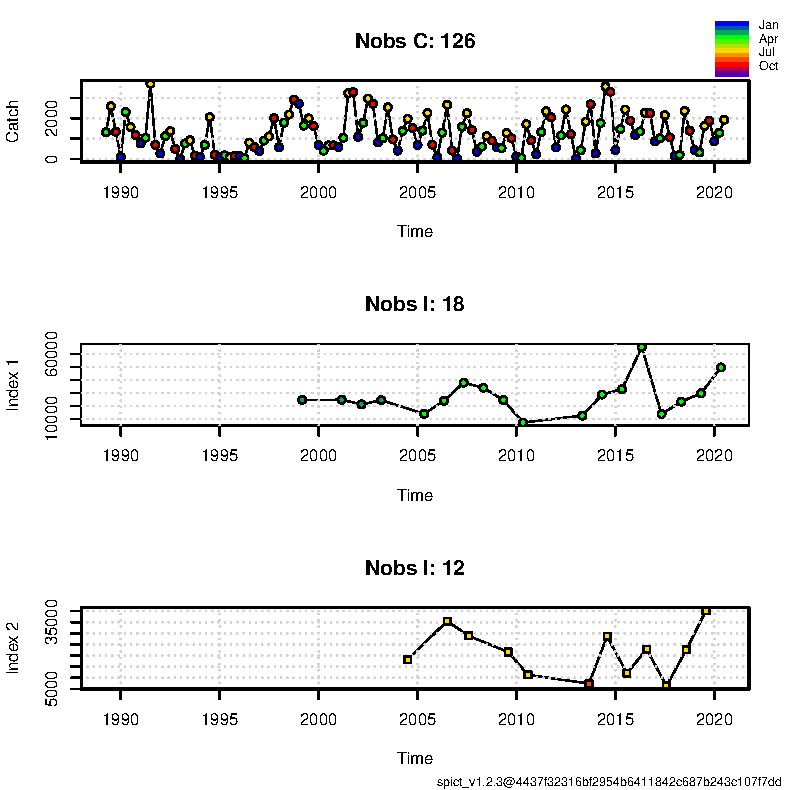
\includegraphics[]{./data.pdf}
 % lendist.pdf: 667x841 pixel, 72dpi, 23.53x29.67 cm, bb=0 0 667 841
 \caption{Summary of data used for the SPiCt model}
 \label{spdata}
\end{figure}


\section{Scenarios}

Four different scenarios were tested, the first one with no seasonal productivity, the second one assuming seasonal productivity, the third one with no seasonal productivity and with time-varying growth and the last one with no seasonal productivity, no time-varying growth and with the data restricted to the 1999-2019 period where there is a more stable length distribution pattern.

\section{Results}

\subsection{Scenario 1}
Most important outputs for scenario 1 are displayed in figure \ref{scenario1out}. This scenario assumes no seasonal productivity, no time-varying growth and uses the whole data set available. Diagnostics are displayed in figure \ref{diag1} and the following is the results summary:





\begin{figure}[h!]
 \centering
 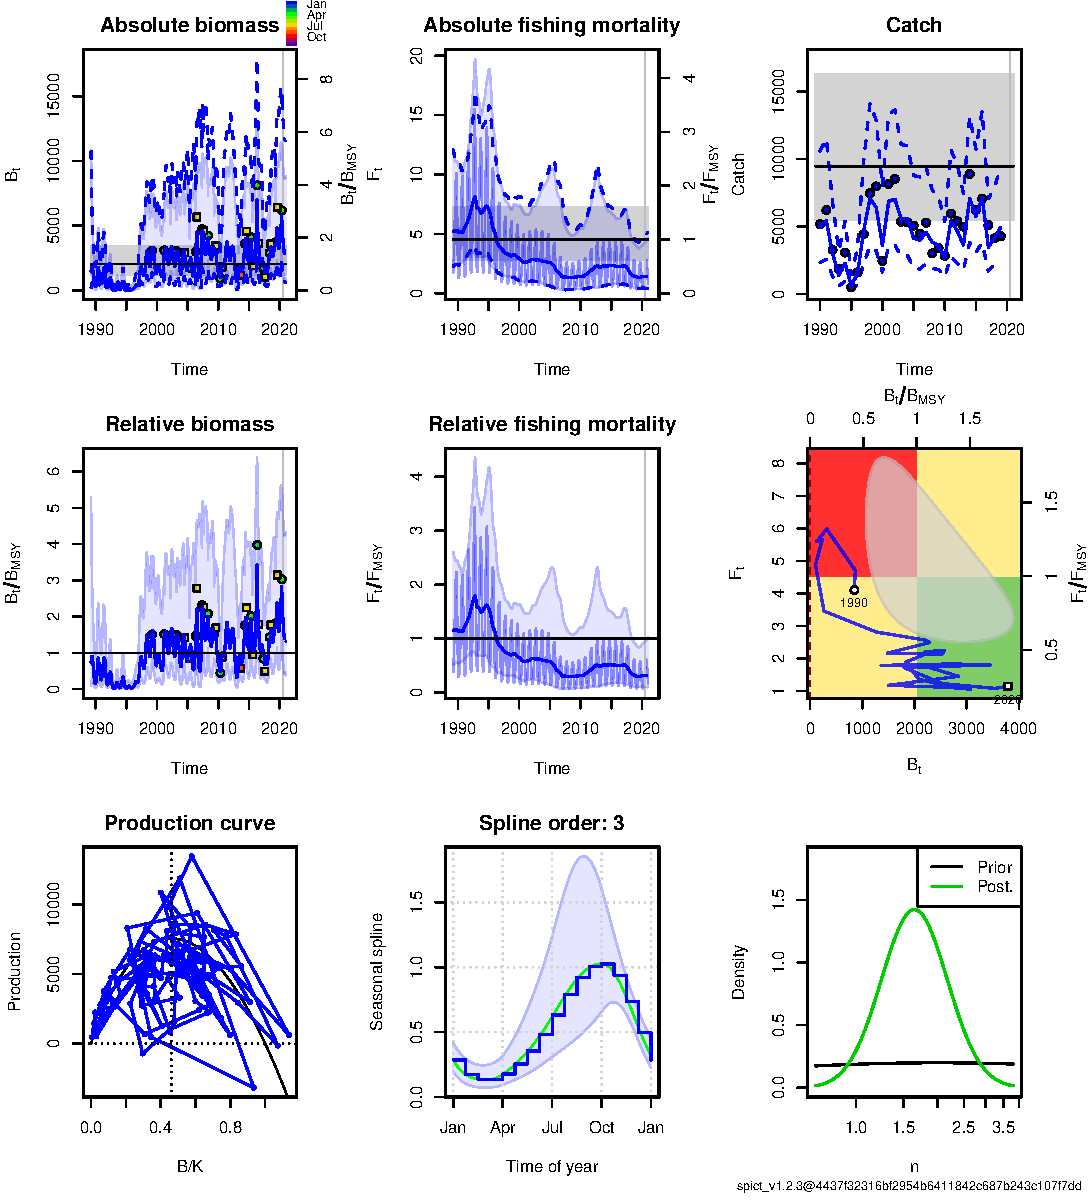
\includegraphics[]{./scenario1out.pdf}
 % lendist.pdf: 667x841 pixel, 72dpi, 23.53x29.67 cm, bb=0 0 667 841
 \caption{Summary of SPiCt results for scenario 1}
 \label{scenario1out}
\end{figure}

\begin{figure}[h!]
 \centering
 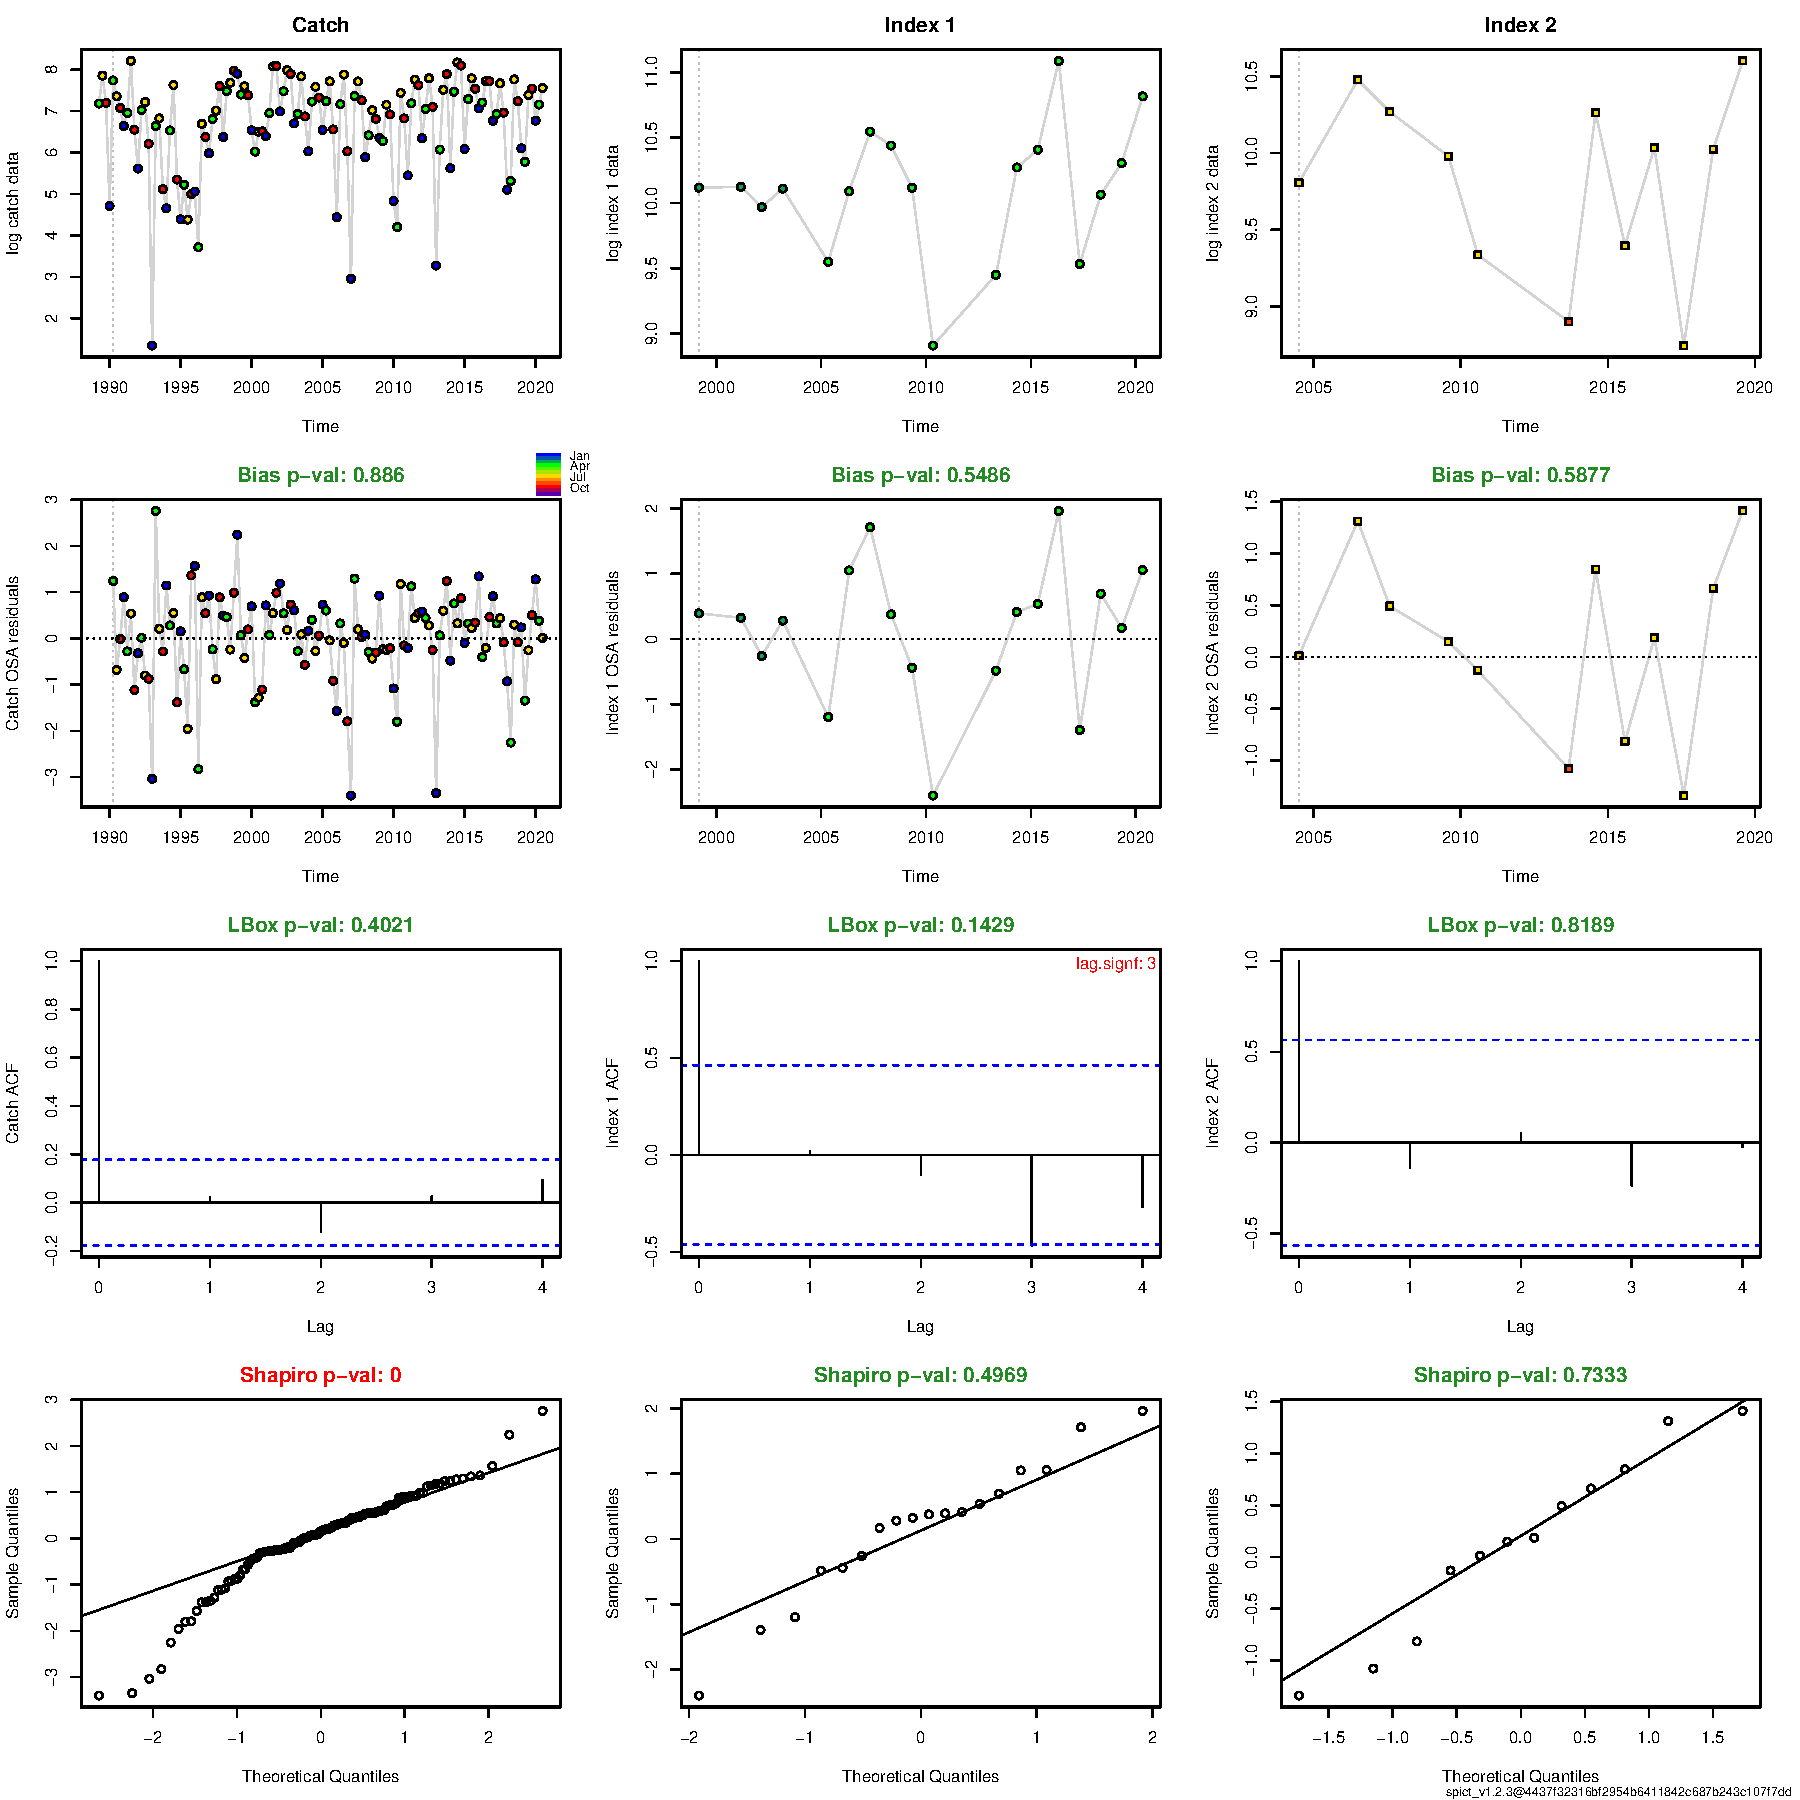
\includegraphics[]{./scenario1diag.pdf}
 % lendist.pdf: 667x841 pixel, 72dpi, 23.53x29.67 cm, bb=0 0 667 841
 \caption{Summary of SPiCt diagnostics for scenario 1}
 \label{diag1}
\end{figure}

\clearpage
\subsection{Scenario 2}
Most important outputs for scenario 2 are displayed in figure \ref{scenario2out}. This scenario assumes a seasonal productivity, no time-varying growth and uses the whole data set available. No diagnostics are available because of the lack of convergence, nevertheless, a plot on how the model estimates the seasonal productivity pattern is presented in figure \ref{seaprod}. The following is the results summary:

\begin{Schunk}
\begin{Soutput}
null device 
          1 
\end{Soutput}
\end{Schunk}


\begin{figure}[h!]
 \centering
 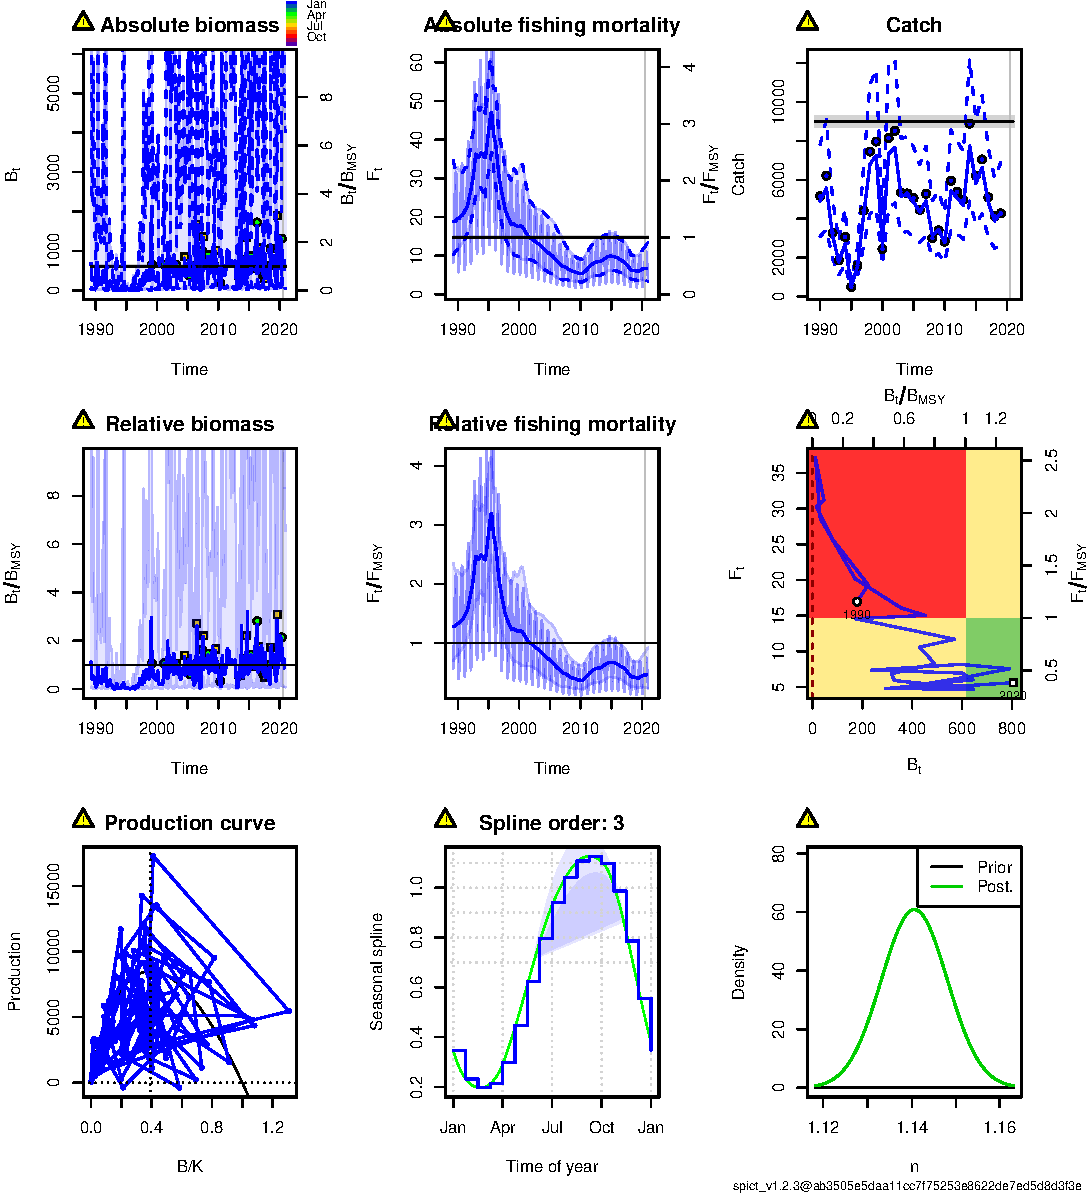
\includegraphics[]{./scenario2out.pdf}
 % lendist.pdf: 667x841 pixel, 72dpi, 23.53x29.67 cm, bb=0 0 667 841
 \caption{Summary of SPiCt results for scenario 2}
 \label{scenario2out}
\end{figure}

% \begin{figure}[h!]
%  \centering
%  \includegraphics[]{./scenario2diag.pdf}
%  % lendist.pdf: 667x841 pixel, 72dpi, 23.53x29.67 cm, bb=0 0 667 841
%  \caption{Summary of SPiCt diagnostics for scenario 2}
%  \label{diag2}
% \end{figure}

\begin{figure}[h!]
 \centering
 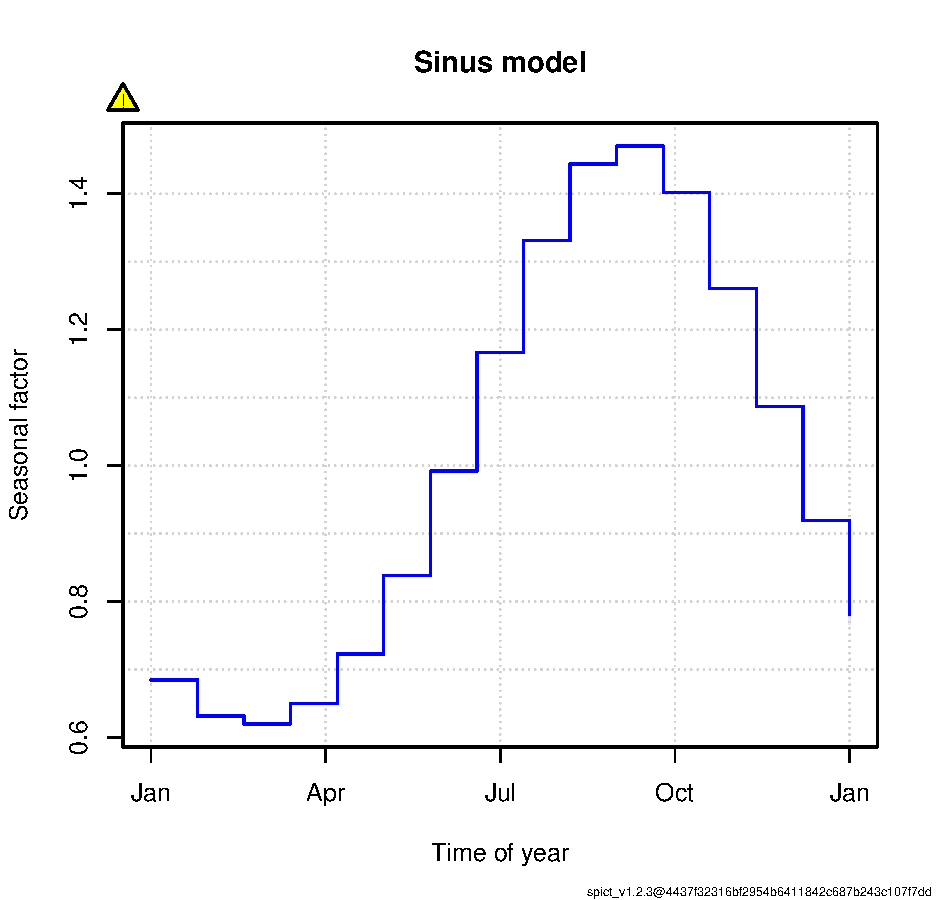
\includegraphics[]{./seaprod.pdf}
 % lendist.pdf: 667x841 pixel, 72dpi, 23.53x29.67 cm, bb=0 0 667 841
 \caption{Estimation of the seasonal productivity pattern in scenario 2}
 \label{seaprod}
\end{figure}




\clearpage

\subsection{Scenario 3}
Most important outputs for scenario 3 are displayed in figure \ref{scenario3out}. This scenario assumes no seasonal productivity, time-varying growth and uses the whole data set available. Diagnostics are displayed in figure \ref{diag3} and the following is the results summary:



% \begin{figure}[h!]
%  \centering
%  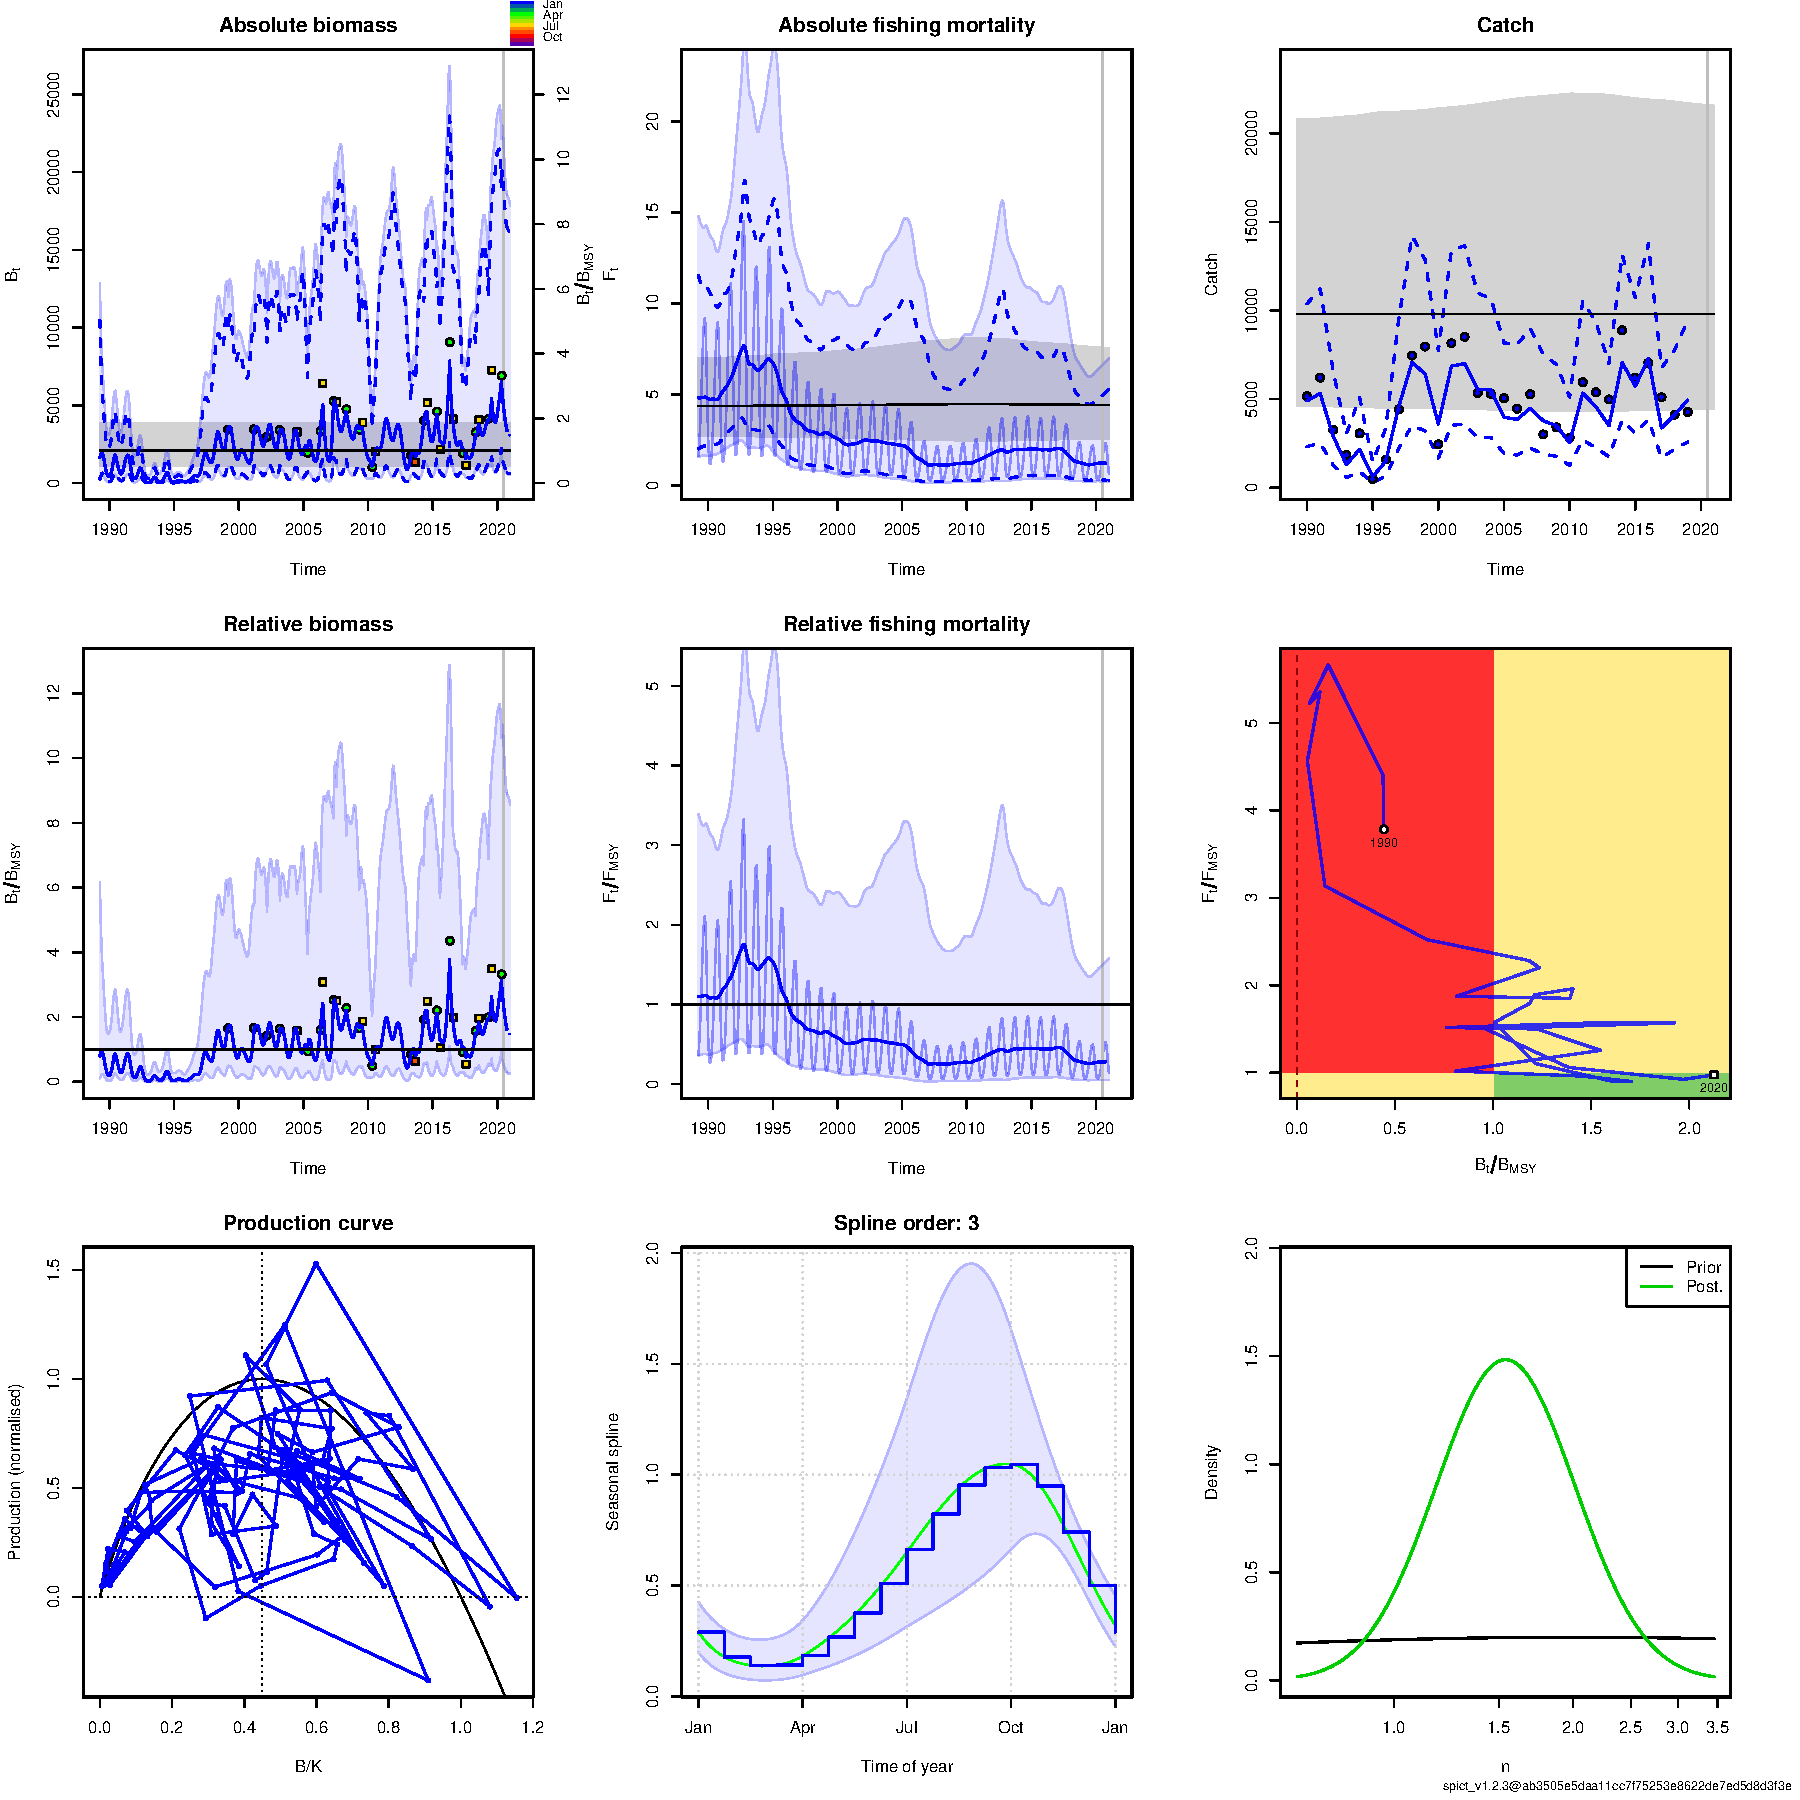
\includegraphics[]{./scenario3out.pdf}
%  % lendist.pdf: 667x841 pixel, 72dpi, 23.53x29.67 cm, bb=0 0 667 841
%  \caption{Summary of SPiCt results for scenario 3}
%  \label{scenario3out}
% \end{figure}

\begin{figure}[h!]
 \centering
 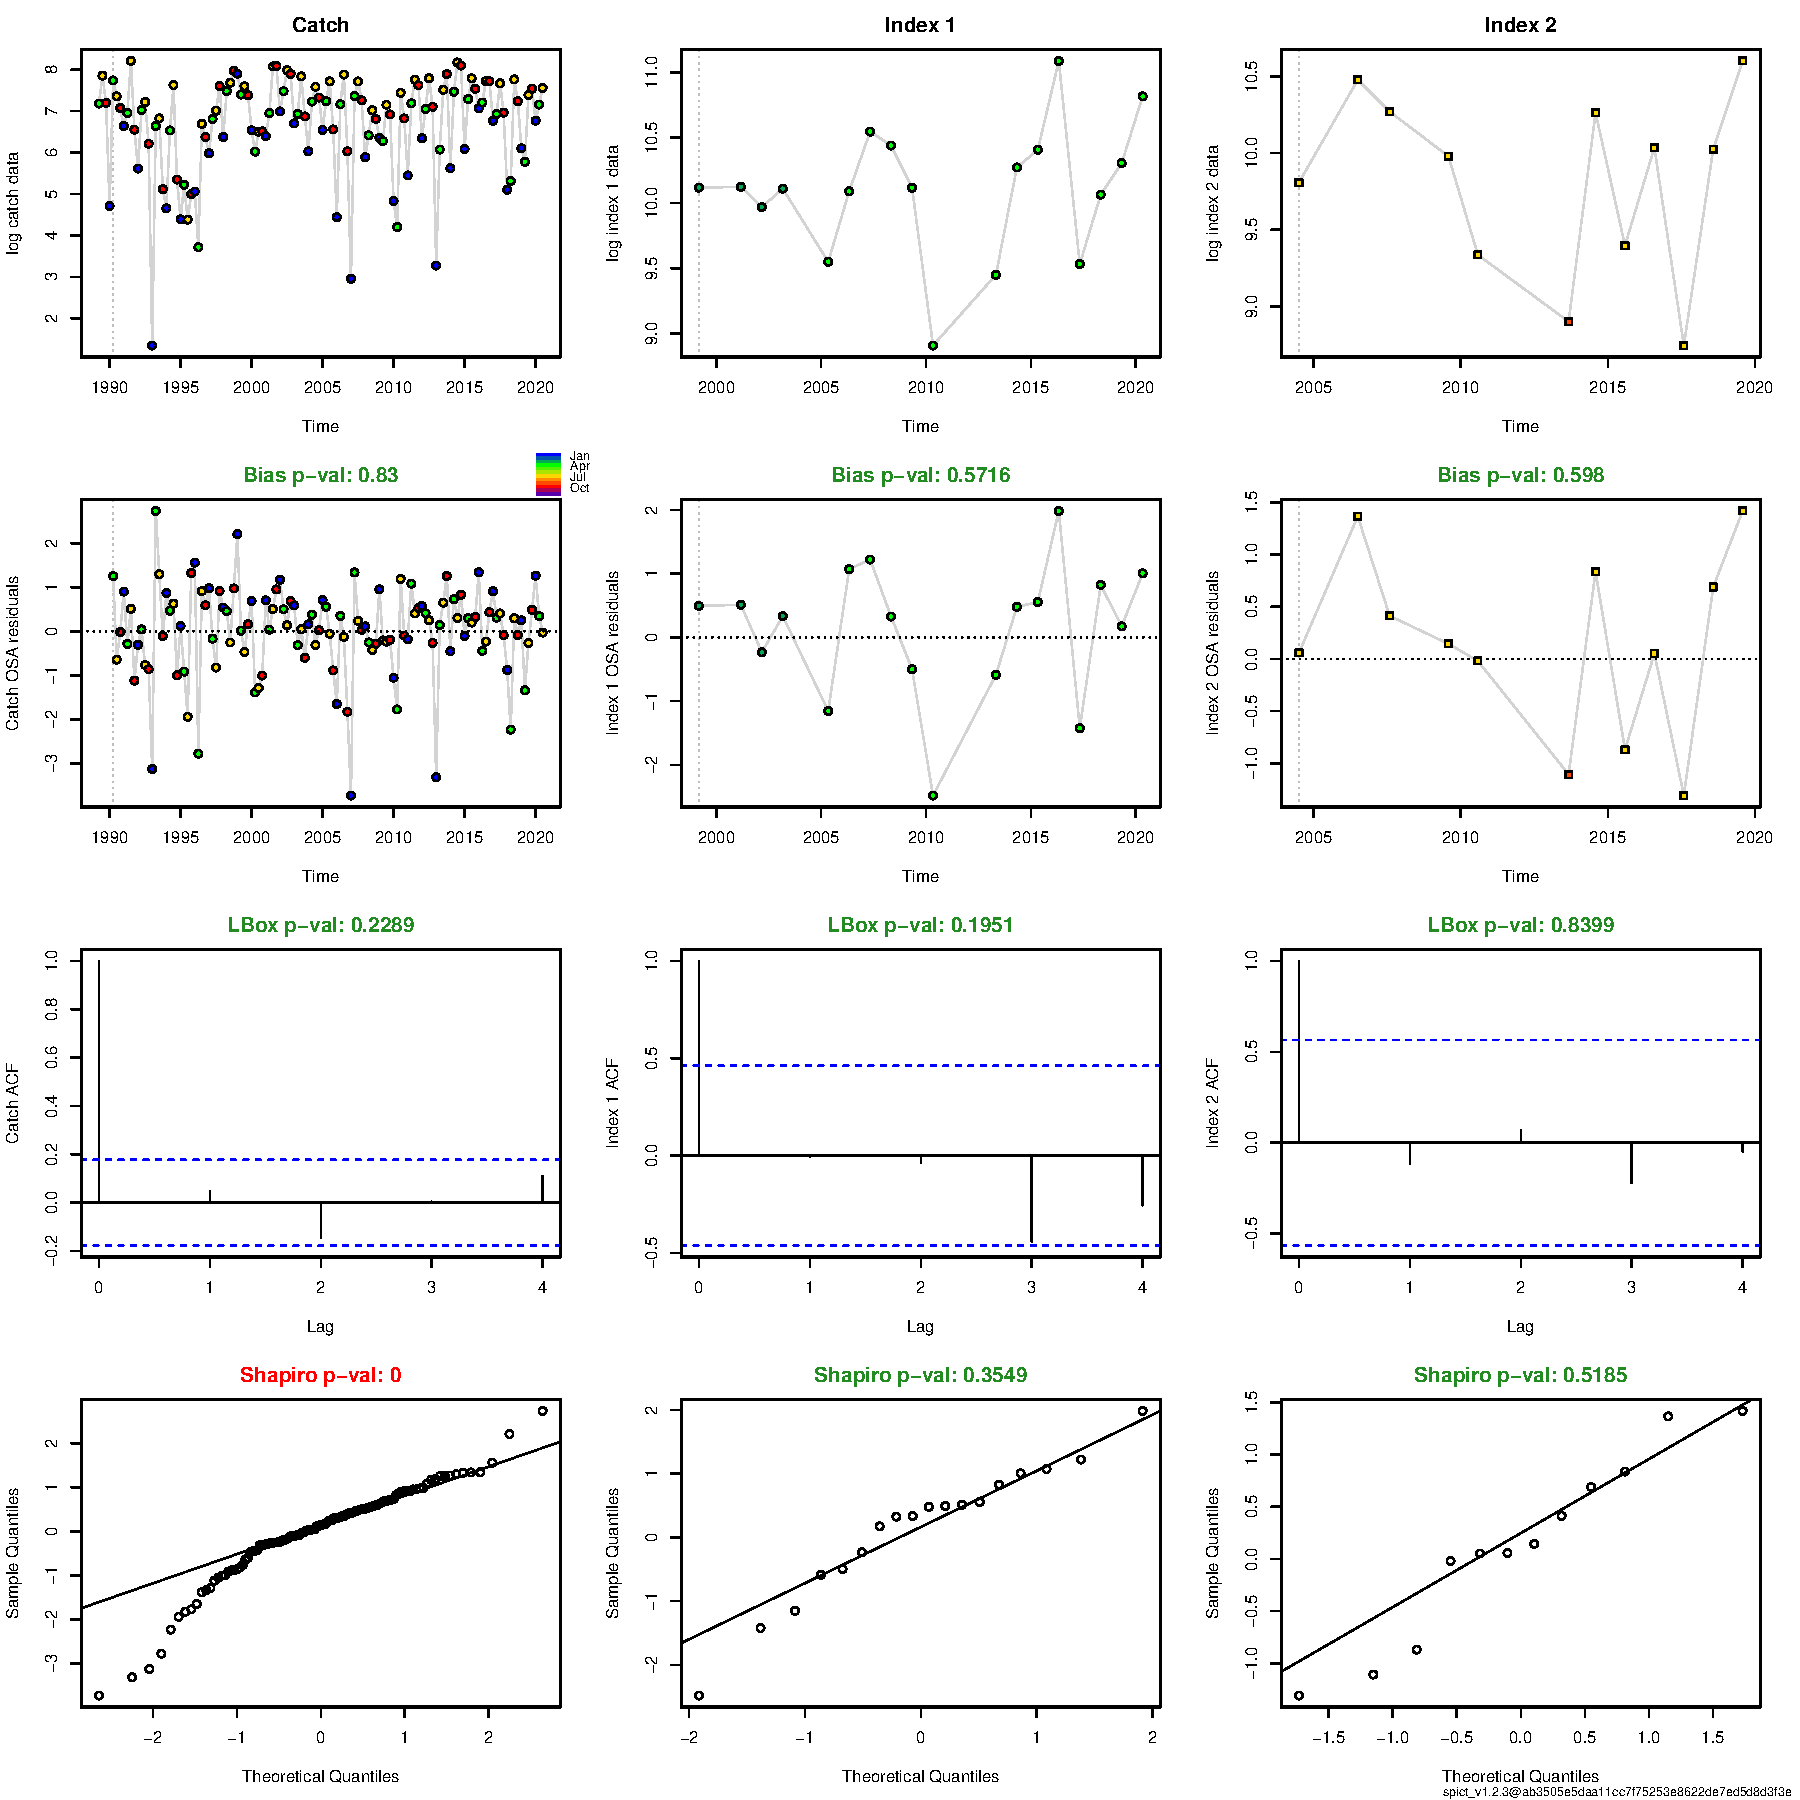
\includegraphics[]{./scenario3diag.pdf}
 % lendist.pdf: 667x841 pixel, 72dpi, 23.53x29.67 cm, bb=0 0 667 841
 \caption{Summary of SPiCt diagnostics for scenario 3}
 \label{diag3}
\end{figure}
\clearpage
\subsection{Scenario 4}
Most important outputs for scenario 4 are displayed in figure \ref{scenario4out}. This scenario assumes no seasonal productivity, no time-varying growth and uses a restricted dataset, with data only for the 1999-2019 period where there is a more stable length distribution pattern. Diagnostics are displayed in figure \ref{diag4} and the following is the results summary:



\begin{figure}[h!]
 \centering
 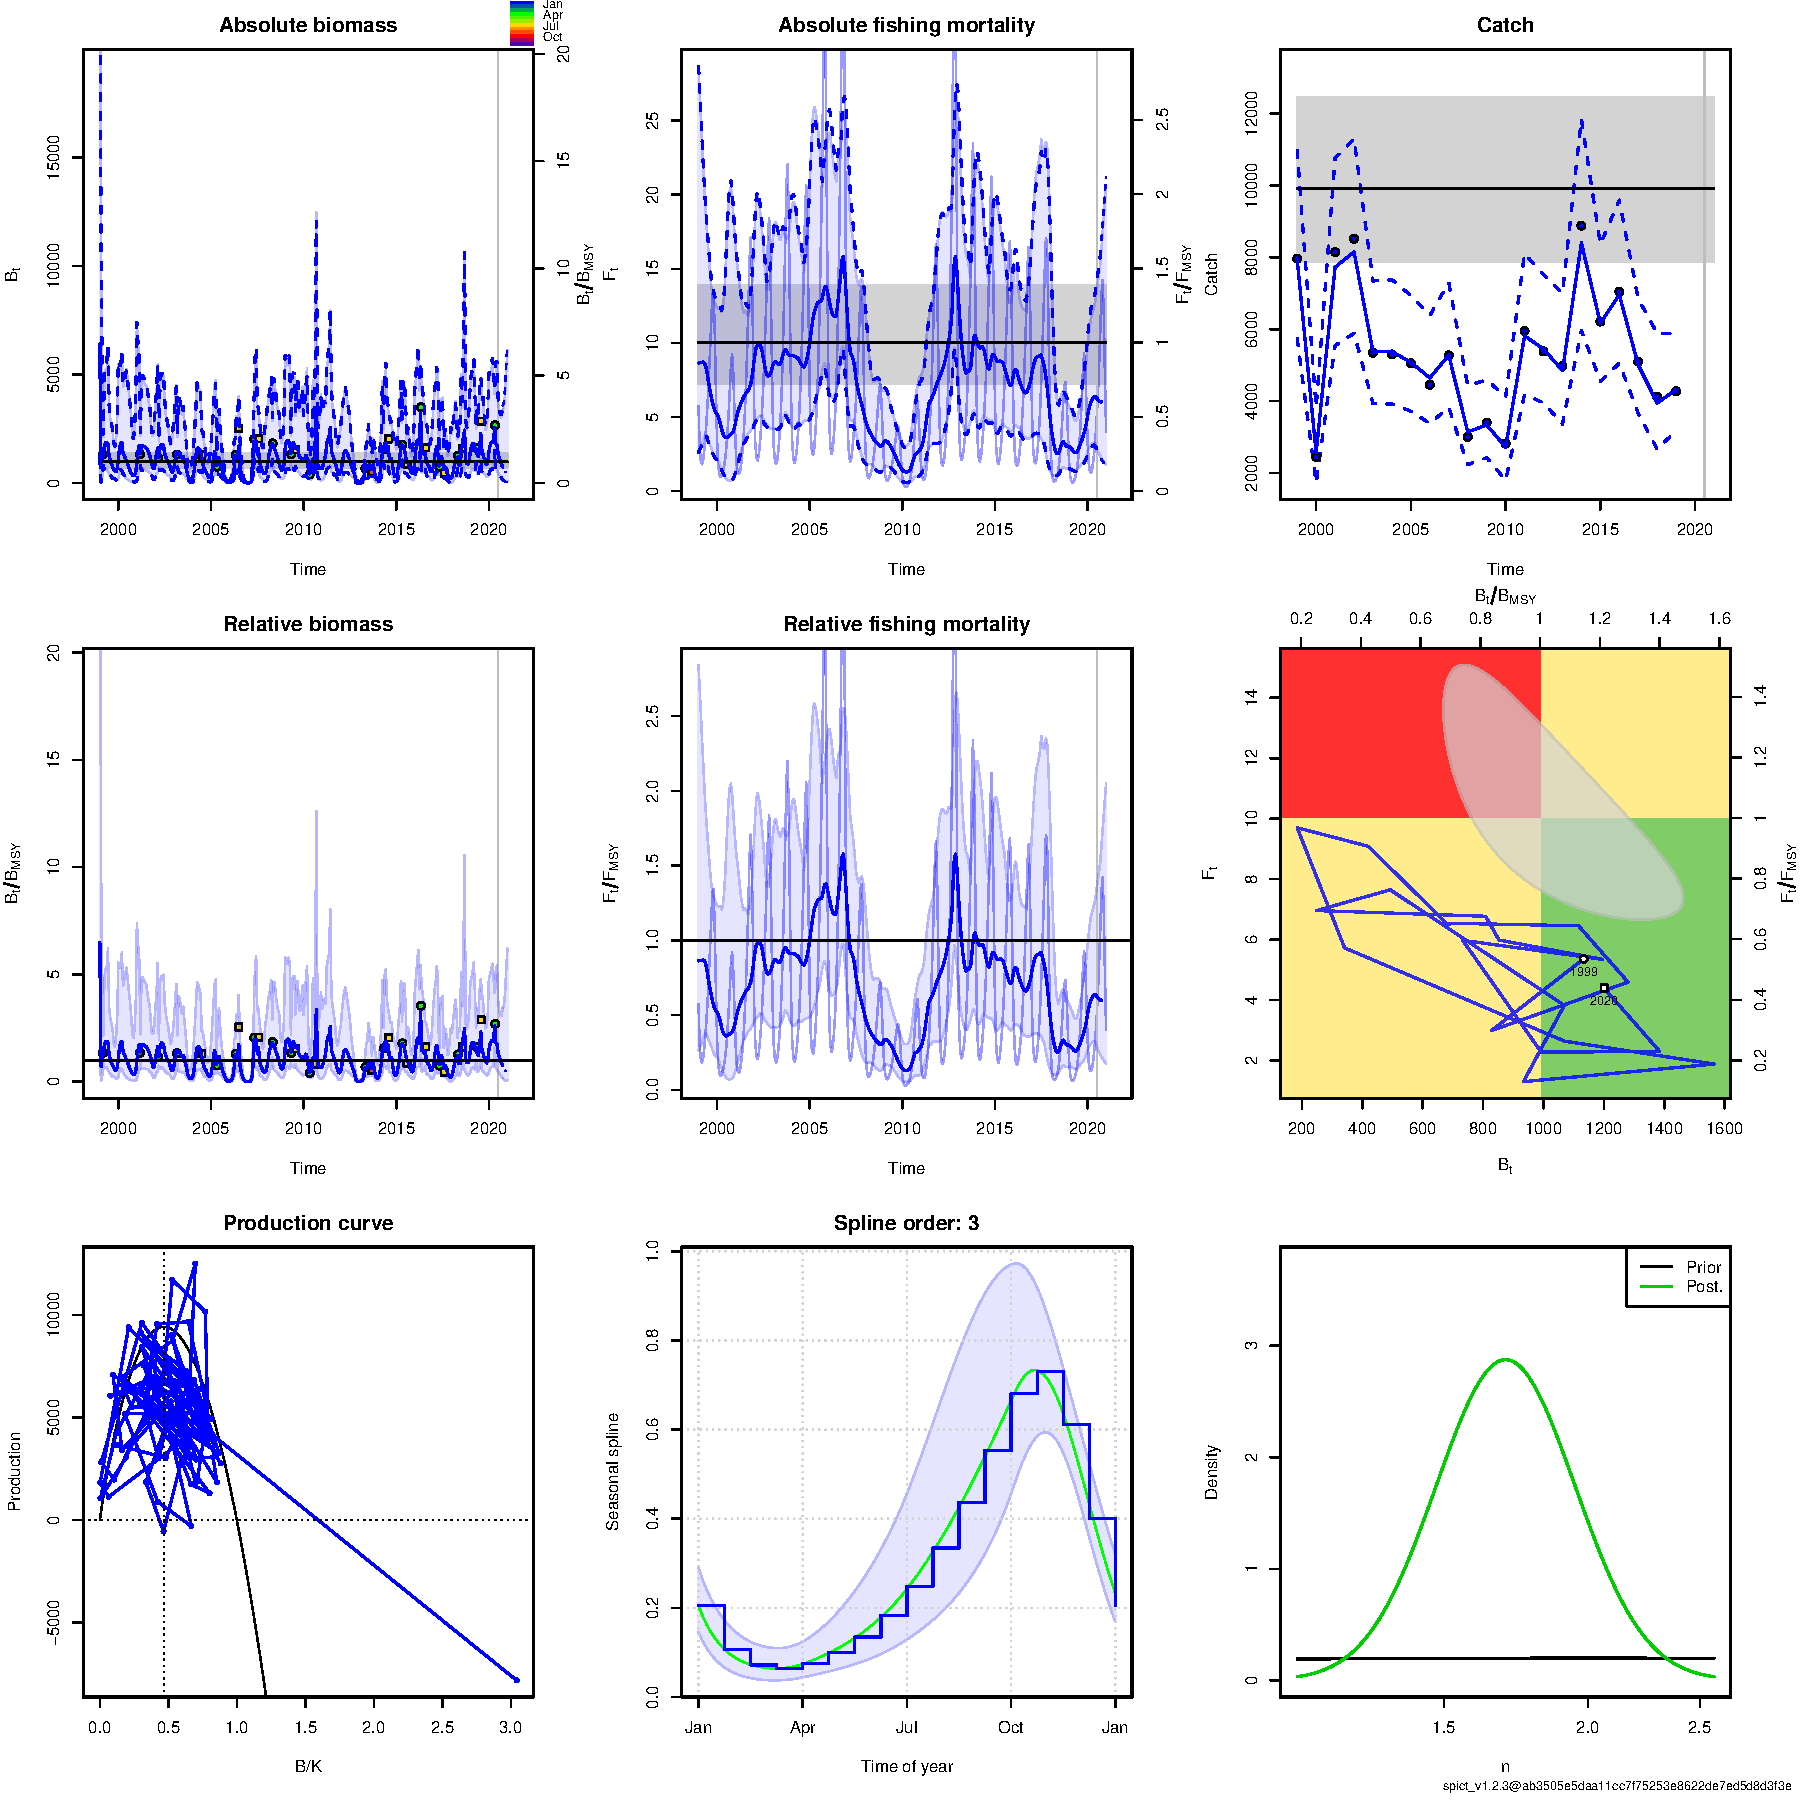
\includegraphics[]{./scenario4out.pdf}
 % lendist.pdf: 667x841 pixel, 72dpi, 23.53x29.67 cm, bb=0 0 667 841
 \caption{Summary of SPiCt results for scenario 4}
 \label{scenario4out}
\end{figure}

\begin{figure}[h!]
 \centering
 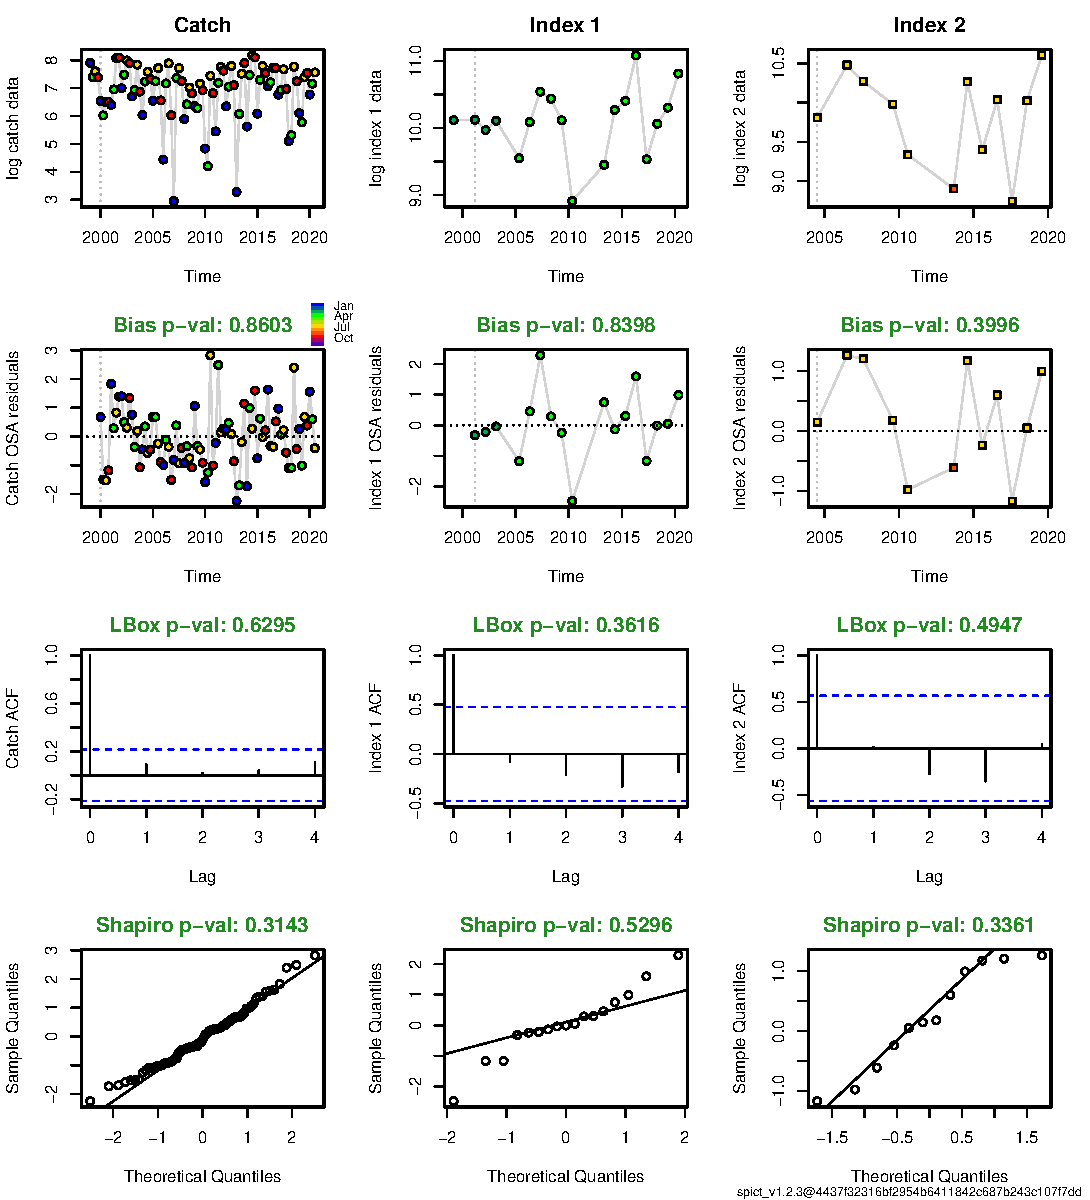
\includegraphics[]{./scenario4diag.pdf}
 % lendist.pdf: 667x841 pixel, 72dpi, 23.53x29.67 cm, bb=0 0 667 841
 \caption{Summary of SPiCt diagnostics for scenario 4}
 \label{diag4}
\end{figure}

\clearpage
\section{Scenario 1 detailed model output}
According to the previous plots, scenario 1 results are more consistent regarding uncertainty intervals and diagnostics, thus more detailed information about its output is presented 

\begin{Schunk}
\begin{Sinput}
> summary(fit1)
\end{Sinput}
\begin{Soutput}
Convergence: 0  MSG: relative convergence (4)
Objective function at optimum: 191.5553781
Euler time step (years):  1/16 or 0.0625
Nobs C: 126,  Nobs I1: 18,  Nobs I2: 12

Residual diagnostics (p-values)
    shapiro   bias    acf   LBox shapiro bias acf LBox  
 C   0.0000 0.8860 0.1848 0.4021     ***    -   -    -  
 I1  0.4969 0.5486 0.0474 0.1429       -    -   *    -  
 I2  0.7333 0.5877 0.4134 0.8189       -    -   -    -  

Priors
     logn  ~  dnorm[log(2), 2^2]
 logalpha  ~  dnorm[log(1), 2^2]
  logbeta  ~  dnorm[log(1), 2^2]

Model parameter estimates w 95% CI 
            estimate        cilow        ciupp    log.est  
 alpha1    0.1500161    0.0263926 8.526944e-01 -1.8970130  
 alpha2    0.2581998    0.0691201 9.645113e-01 -1.3540214  
 beta      1.9976305    0.8534965 4.675506e+00  0.6919617  
 r         5.5785227    1.7461581 1.782193e+01  1.7189240  
 rc        6.7973357    3.0766562 1.501753e+01  1.9165307  
 rold      8.6976185    3.7445113 2.020252e+01  2.1630492  
 m      7573.7985299 4864.6661424 1.179165e+04  8.9324500  
 K      4825.5323568 2080.7202763 1.119120e+04  8.4816763  
 q1        8.0511334    3.5635780 1.818979e+01  2.0858129  
 q2        6.2595990    2.6129244 1.499568e+01  1.8341161  
 n         1.6413851    0.9472899 2.844055e+00  0.4955404  
 sdb       1.2003848    0.6501406 2.216326e+00  0.1826422  
 sdf       0.3130694    0.1375802 7.124024e-01 -1.1613303  
 sdi1      0.1800770    0.0363820 8.913131e-01 -1.7143708  
 sdi2      0.3099392    0.1029656 9.329548e-01 -1.1713792  
 sdc       0.6253970    0.4919972 7.949667e-01 -0.4693686  
 phi1      0.0819407    0.0386710 1.736256e-01 -2.5017597  
 phi2      0.3789405    0.1822619 7.878550e-01 -0.9703760  
 phi3      1.0525103    0.4532576 2.444036e+00  0.0511781  
 
Deterministic reference points (Drp)
          estimate       cilow        ciupp  log.est  
 Bmsyd 2228.460940 1032.323330  4810.545318 7.709066  
 Fmsyd    3.398668    1.538328     7.508764 1.223383  
 MSYd  7573.798530 4864.666142 11791.646640 8.932450  
Stochastic reference points (Srp)
          estimate       cilow        ciupp  log.est rel.diff.Drp  
 Bmsys 2039.821232 1216.082809  3421.535628 7.620617  -0.09247855  
 Fmsys    4.531853    2.822374     7.276742 1.511131   0.25004892  
 MSYs  9457.933044 5493.907566 16282.126408 9.154609   0.19921208  

States w 95% CI (inp$msytype: s)
                    estimate        cilow        ciupp    log.est  
 B_2020.50      4069.6356432 1179.4259659 1.404237e+04  8.3113088  
 F_2020.50         1.4445672    0.4326156 4.823622e+00  0.3678098  
 B_2020.50/Bmsy    1.9950943    0.7929830 5.019529e+00  0.6906913  
 F_2020.50/Fmsy    0.3187586    0.1070864 9.488324e-01 -1.1433211  

Predictions w 95% CI (inp$msytype: s)
                  prediction       cilow        ciupp    log.est  
 B_2020.75      2844.3262034 690.0175239 1.172462e+04  7.9530815  
 F_2020.75         1.4438795   0.4171718 4.997433e+00  0.3673336  
 B_2020.75/Bmsy    1.3943997   0.4571585 4.253121e+00  0.3324640  
 F_2020.75/Fmsy    0.3186069   0.1029483 9.860323e-01 -1.1437973  
 Catch_2020.75  1453.1820191 629.9886794 3.352025e+03  7.2815109  
 E(B_inf)       3381.8325751          NA           NA  8.1261730  
\end{Soutput}
\end{Schunk}


\section{Comparison of harvestable biomass estimation obtained in scenario 1 with harvestable biomass estimated by Gadget}







Figures \ref{comp_abs} and \ref{comp} show model comparison estimates of absolute (in tonnes) and relative harvestable biomass at the end of the second quarter, respectively. The models used for this comparison are, the SPiCt scenario 1  and the Gadget model used in the latest anchovy 9a South assessment \citep{Rincon20}. The data used for the SPiCt scenario was also the same used in this assessment. In Figure \ref{comp_abs} it can be observed that the two models present different trends mostly before 2005 (the year when PELAGO survey starts). A comparison between SPiCt estimates of harvestable biomass with catches time series (Figure \ref{spict_catches}) suggest that catches time series have a big influence on the SPiCT estimates.
\begin{figure}[h!]
 \centering
 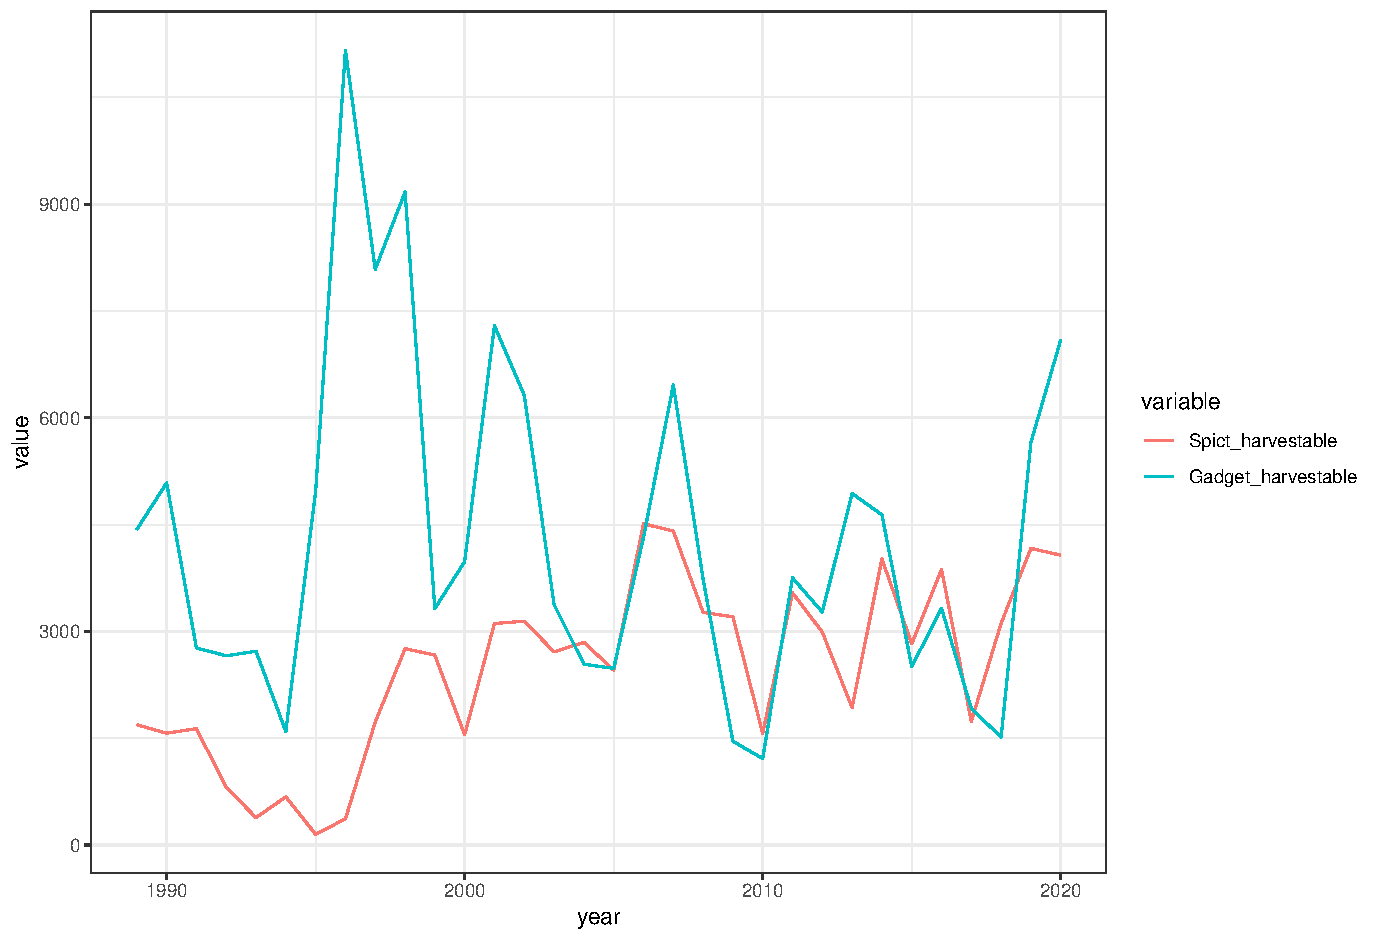
\includegraphics[]{./comparison_abs.pdf}
 % lendist.pdf: 667x841 pixel, 72dpi, 23.53x29.67 cm, bb=0 0 667 841
 \caption{Comparison of absolute harvestable biomass estimates at the end of the second quarter of each year by Spict (scenario 1) and Gadget, pink and blue lines, respectively.}
 \label{comp_abs}
\end{figure}




\begin{figure}[h!]
 \centering
 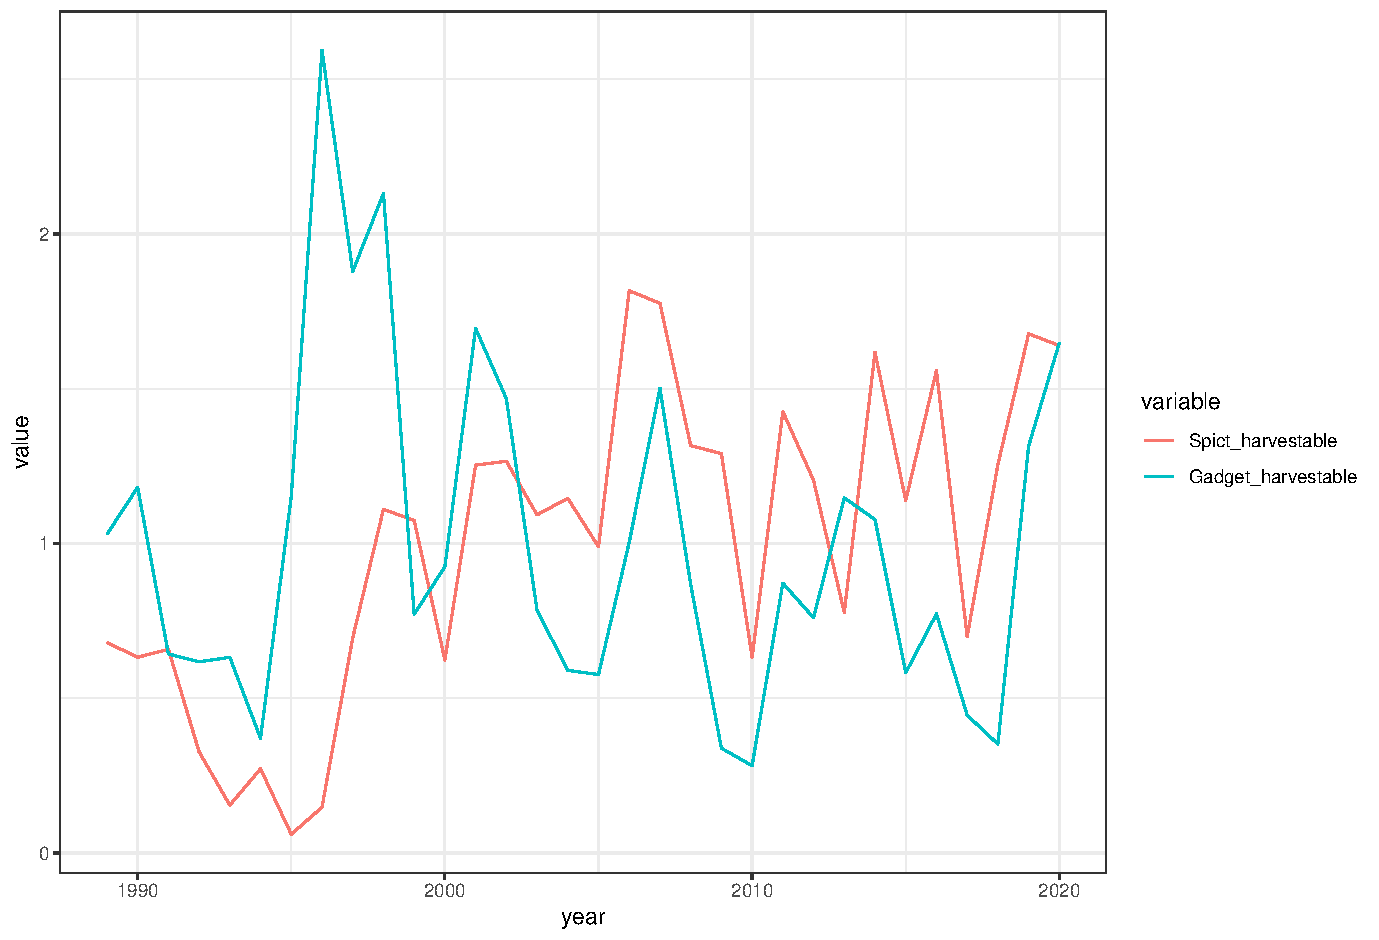
\includegraphics[]{./comparison.pdf}
 % lendist.pdf: 667x841 pixel, 72dpi, 23.53x29.67 cm, bb=0 0 667 841
 \caption{Comparison of relative harvestable biomass estimates at the end of the second quarter of each year by Spict (scenario 1) and Gadget, pink and blue lines, respectively.}
 \label{comp}
\end{figure}

\begin{figure}[h!]
 \centering
 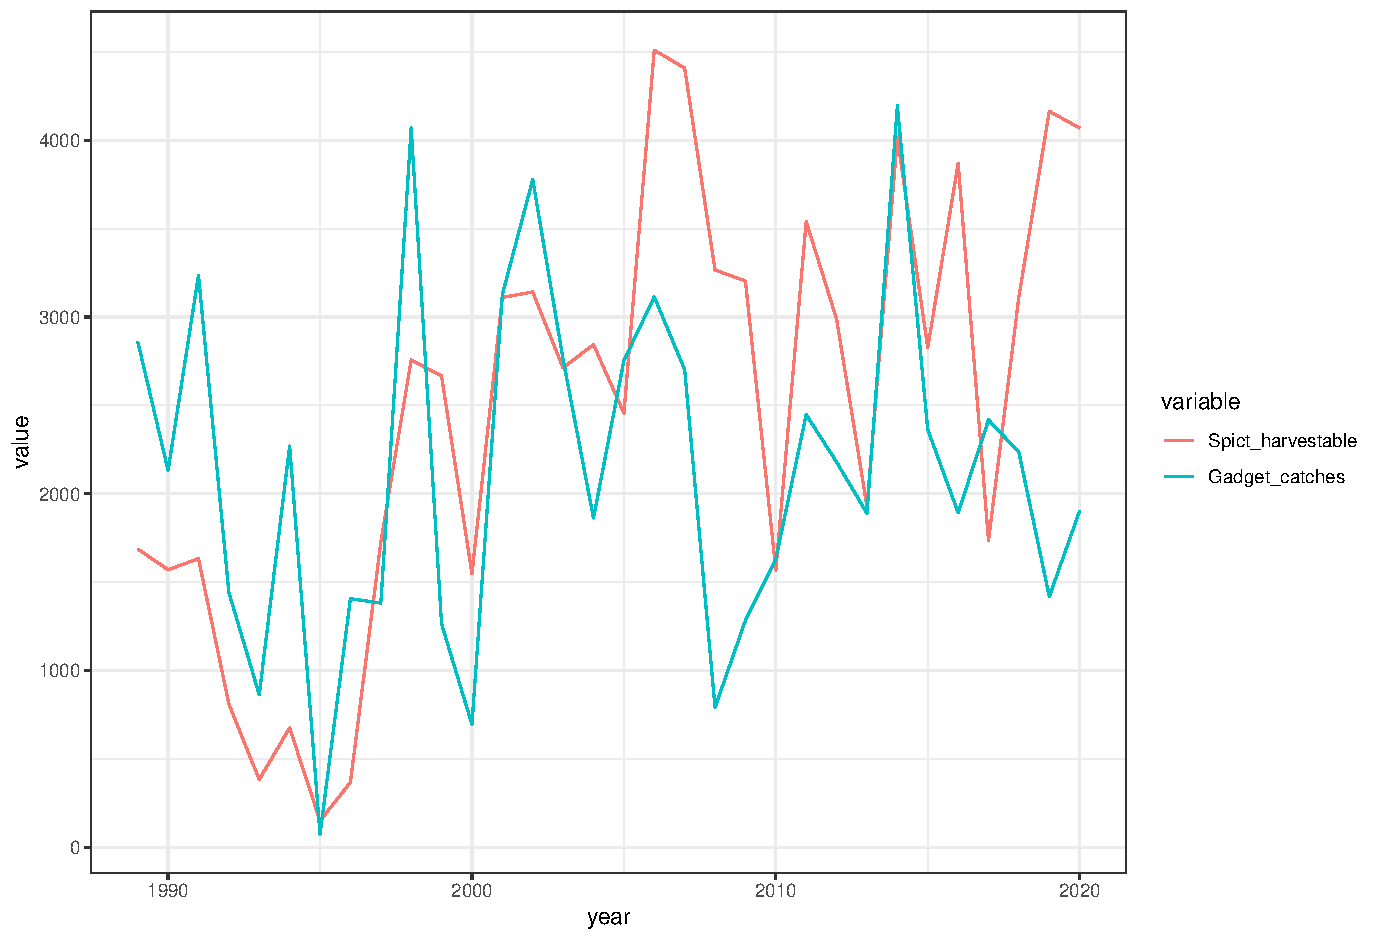
\includegraphics[]{./comparison_abs_biospict_gadgetcatches.pdf}
 % lendist.pdf: 667x841 pixel, 72dpi, 23.53x29.67 cm, bb=0 0 667 841
 \caption{Comparison of absolute harvestable biomass estimates at the end of the second quarter of each year by Spict (scenario 1) and catches time series, pink and blue lines, respectively.}
 \label{spict_catches}
\end{figure}



\clearpage
\section{References}

\bibliography{totalfv,Granger,paper1,paper1zotero,RUIZetal,paper2,total}


\end{document}














% \begin{figure}[h!]
%  \centering
%  \includegraphics[bb=0 0 662 451]{./biomassts.pdf}
%  % lendist.pdf: 667x841 pixel, 72dpi, 23.53x29.67 cm, bb=0 0 667 841
%  \caption{Estimated biomass time series at the end of quarter two (Age 0 removed to be consistent with recruitment at the end of the second quarter of the year). Note that under the assumption that all individuals in $B1+$ class are mature, this biomass is equivalent to SSB}
%  \label{biomassts}
% \end{figure}

% \section{Catch advice for July 2018 to June 2019}
% 


%3443 capturas algarve y españa 2018 2383.25045 seún Fernando
%para 2017 catches segundo semestre 1224.3816 más discards 122.483

%Para las capturas totales revisar el estesi3_fv_local en GADGET/Assessment/Assessment2018
% TOTALCATCHfv
%       Col1
% 1 3607.638 + discards

%2019 Advice
% \section{Catch advice for July 2019 to June 2020}
% 
% 

% 
% 

% 


% %where $B$ represents the estimated abundance by the model as shown in Figure \ref{biomassts}
% \section{Reference points}
% 
% The methodology applied was the same decided in WKPELA 2018 (page 286 of WKPELA 2018 report (ICES, 2018)) following ICES guidelines for calculation of reference points for category 1 and 2 stocks and the report of the workshop to review the ICES advisory framework for short lived species ICES WKMSYREF5 2017 (ICES, 2017).
% 

% %Note that we are now using 2010 as reference for $Bloss$ instead of 2010 as was done during WKPELA 2018, this is because we found some inconsistencies in the maturity ogives used, and we now assume age 1+ individuals ($B_1+$) as mature (see subsection \ref{ARF} above)
% %está en tons 
% 
% ICES recommends to calculate $Bpa$ as follows: $$Bpa = e^{(1.645\sigma)} Blim,$$

% 
% 
% 
% %  ICES
% % uses Bpa = 1.4 Blim for many of the longer-lived stocks (1.4 is an upward rounding of
% % e
% % 1.645
% % , where =0.2), and it was suggested that a candidate default value for short-lived
% % stocks could be σ0.3 (approximately the average of the values in Table 3.2.1) corresponding
% % to Bpa = 1.64 Blim
% 
% 
% 
% 



% \begin{figure}[h!]
%  \centering
%  \includegraphics[bb=0 0 595 288]{./SSBt_1rect.pdf}
%  % lendist.pdf: 667x841 pixel, 72dpi, 23.53x29.67 cm, bb=0 0 667 841
%  \caption{Estimated Stock Spawning biomass ($SSB_{t}$) vs. Recruitment ($R_{t}$), $SSB_{t}$ corresponds to the Stock Spawning Biomass at the end of quarter 2 of year $t$, while $R_{t}$ corresponds to the sum of the recruitment at the beginning of quarters 3,4 and 1 of years $t$ and $t+1,$ respectively.}
%  \label{SSBt_1rect}
% \end{figure}
% 
% 


% \begin{figure}[h!]
%  \centering
%  \includegraphics[bb=0 0 595 288]{./discharges88_15Hm3month.pdf}
%  % discharges88_15Hm3month.pdf: 595x288 pixel, 72dpi, 20.99x10.16 cm, bb=0 0 595 288
%  \caption{Quaterly accumulated cubic hectometers that are discharged from Alcalá del Río dam in logarithmic scale.}
%  \label{Displot}
% \end{figure}





%Total mortality $Z$ was approximated using catch at age data with the following equation: $$\log(\frac{C_{1}^{y-1}}{C_{2}^{y}}), y=1990,\dots,2016,$$ where $C_{a}^{y}$ denotes catches in numbers at age $a$ during year $y.$ The results are presented in Figure \ref{Ffromcatches}. Analogously, the same estimation was performed using the age data provided by the ECOCADIZ survey and the results are presented in Figure \ref{Zfromecocadiz}.

%Estimated F for age 1, mean estimated F for Ages 1 and 2 and estimated $Z_{1,2}$ are presented in figure \ref{F1_F12_Z12}.

%High values for $F$ are consistent with the values of $\log(\frac{C_{1}^{y-1}}{C_{2}^{y}}), y=1989,\dots,2015$ where $C_{a}^{y}$ denotes catches in numbers at age $a$ during year $y,$ (see Figure \ref{Ffromcatches}).
% \begin{figure}[h!]
%  \centering
%  \includegraphics[bb=0 0 595 288]{./Ffromcatches.pdf}
%  \caption{Estimation of Z using information from yearly catch in numbers from individuals of age 1 and 2.}
%  % Ffromcatches.pdf: 307x288 pixel, 72dpi, 10.83x10.16 cm, bb=0 0 307 288
%  \label{Ffromcatches}
% \end{figure}
% 
% \begin{figure}[h!]
%  \centering
%  \includegraphics[bb=0 0 595 288]{./Zfromecocadiz.pdf}
%  \caption{Estimation of Z using information from ECOCADIZ age samples from individuals of age 1 and 2.}
%  % Ffromcatches.pdf: 307x288 pixel, 72dpi, 10.83x10.16 cm, bb=0 0 307 288
%  \label{Zfromecocadiz}
% \end{figure}

% \begin{figure}[h!]
%  \centering
%  \includegraphics[bb=0 0 518 432]{./F1_F12_Z12.pdf}
%  \caption{Estimated F for age 1, mean estimated F for Ages 1 and 2 and estimated $Z_{1,2}$ }
%  \label{F1_F12_Z12}
%  % ICESplots.pdf: 523x379 pixel, 72dpi, 18.45x13.37 cm, bb=0 0 523 379
% \end{figure}

% \section{Scenarios to explore}
% \begin{enumerate}
% \item Natural mortality obtained by expert elicitation $M_{0}=1.5, M_{1}=1, M_{2}=1.5, M_{3}=1:$ A bad fitting was obtained showing the sensitivity of the model results to this value. Some variations of this scenario should be explored.
% \item Natural mortality at age estimated by the model
% \item Forecast assuming that the advice is provided:
% \begin{itemize}
% %\item In February of year ‘y+1’ for year ’y+1’ including all the available surveys indices (i.e. for recruitment informed on estimates from ECOCADIZ-RECLUTAS). 
% %\item In June of year ‘y’ for year ‘y+1’ without consider the estimates provided by that survey (i.e. for an assumed scenario of recruitment-uninformed by surveys). 
% \item In June of year ‘y’ for year ‘y+1’ %without consider the estimates provided by that survey and updated in April/May of year 'y+1' by 
% including the PELAGO survey performed in March/April.
% \end{itemize}
% \end{enumerate}
% % The results of the Gadget model presented in the Appendix and in Figure \ref{ICESplot} provides valuable information about the status of the stock,  even not accounting for the influence of environmental covariates on recruitment. From Figure \ref{ICESplot}, it could be claimed that high values of fishing mortality seems to appear as a result of an increase of recruitment (1998, 2002) or as previously stated in \citep{ruiz_biological_2017}  as a result of the fixed quota management where $F$ tends to increase where the recruitment is low (1994, 2004, 2007, 2010) and viceversa (1996, 2011). The model confirms the  BotTop population dynamics regime described before in \citet{ruiz_anchovy_2007} where recruitment is transfered from one year to the next,  together with a very high annual exploitation rate (Between 1 and 4, Figure \ref{ICESplot}, top right panel) that hampers them to survive from one year to the next. In particular, we can see that Gadget explains 1995 collapse as a consequence of a bad %
%recruitment and huge $F$ on the previous year. The trend of abundance estimation is also coherent with the one estimated in \citet{ruiz_bayesian_2009}, but the scale is different, Gadget model yearly abundace estimates are between 0 and 750 millions while the other model quarterly estimates are between 0 and 1500 millions. This difference it is difficult to explain because of the way that fishing mortality ($F$) is accounted in both models, Gadget offers the possibility to estimate $F$ directly in order to make catches forward projections while $F$ is not explicitly defined in the other model, therefore $F$ is easily tracked in Gadget and the estimates are very high while in the other model there is no way to get an output that relates abundance with catches. 
% 







%R
%The final question: How Gadget accounts for the variability added by the environment in stages previous to recruitment?






%This suitability have  used also estimationto be estimated such as 

%Gadget or SS3 are mainly focused in modeling biological processes and their interaction with fishing dynamics 


















%\subsection{Management Strategy Evaluation comparison framework}

%Using the 
% From the recruitment time series modelled with Gadget it is possible to extract a numerical relationship with environmental covariates and make forward projections under different management strategies. This follows from the approach developed by the International Whaling Commission, a management strategy evaluation (MSE) \citep{kirkwood_1997, butterworth and Punt_1999, Kell_2005} that have been extensively used in stock assessment \citep{Kell_2007}.
% 
% 
% 
% 
% The flexibility of this platform allow the analysis of different management scenarios, an and  to provide information on anchovy year classes that constitute the magnitude of the biomass and catches.
% 
% 
% 
% in a robust statistical framework to provide information on year classes.
% 




% dthey have been used separately 
% 
% that can be used together to provide information on year classes
% re isn't an appropriate assessment needs a model that supports the incorporation
% ``the lack of available data on year classes that constitute the bulk of the biomass and catches 
% '' the lack of advice in the last two years \citep{ICES2015} relies on This was due to the lack of 
% available data on year classes that constitute the bulk of the biomass and catches 
% 
% 
% 
% That kind of approach is needed for analysis of anchovy population in the Gulf of Cadiz
% 
% available have estimulate a coherent integration of the information 
% 
% 
% the inclusion 
% of auxiliary  information (i.e. survey indexes, fishing effort, length-weight relationships) in modelling framework have result in
% 
% Estimating likelihood components weights and model parameter optimization as described in \citet{taylor_a_simple_2007} incorporates the information provided by different datasets simultaneously and have been used in multiple fisheries applications
% 
% 
% 
% 
% to estimate parameters have been proved to be useful 
% \section{Front matter}
% 
% The author names and affiliations could be formatted in two ways:
% \begin{enumerate}[(1)]
% \item Group the authors per affiliation.
% \item Use footnotes to indicate the affiliations.
% \end{enumerate}
% See the front matter of this document for examples. You are recommended to conform your choice to the journal you are submitting to.
% 
% \section{Bibliography styles}
% 
% There are various bibliography styles available. You can select the style of your choice in the preamble of this document. These styles are Elsevier styles based on standard styles like Harvard and Vancouver. Please use Bib\TeX\ to generate your bibliography and include DOIs whenever available.
% 
% Here are two sample references: \cite{Feynman1963118,Dirac1953888}.

% \section{Acknowledgements}
% 
% %The research leading to these results has received funding from the European Union Seventh Framework Programme (FP7-KBBE-2013) under the grant agreement 613571/MAREFRAME project and  Margarita M. Rincón was funded by P09-RNM-5358 of the Junta de Andalucía. However, the document does not necessarily reflect EC views and in no way anticipates the Commission's future policy in the area. 
% We thank Jamie Lentin from Shuttlethread for the automatization of data input,  Bjarki Elvarsson for having an open repository with very useful Gadget data processing routines and his valuable help, and to the members of WGHANSA group for their guidance and support.
% 
% We gratefully thank CESGA (Galician Supercomputing Center) for computational time at the FTII Supercomputer and technical assistance.
% 
% 
% 
% 
% 
% 
% 
% 
% 
% 
% 
% 
% 
% %\cleardoublepage
% 
% \section{References}
% 
% \bibliography{totalfv,Granger,paper1,paper1zotero,RUIZetal,paper2,total}
% \end{document}
% \appendix
%\numberwithin{equation}{section}
%\numberwithin{figure}{section}
%\numberwithin{table}{section}
% \section{Model description}
% 
% % Here we present the technical details for the implementation of Gadget and simple models using real and simulated data for the Gulf of Cádiz anchovy stock. Real data were extracted from ICES reports as well as from different records that the Instituto Español de Oceanografía has compiled on this stock along the last decades and simulated data were obtained from the minimum realistic model described in \cite{rincon_economic_2016}. 
% 
% The general Gadget model description and all the options available can be found in Gadget manual \citep{begley_gadget_2004} and some specific examples can be found in \citet{taylor_simple_2007} and \citet{elvarsson_bootstrap_2014}. The Gadget model implementation consists in three parts, a simulation of biological dynamics of the population (simulation model), a fitting of the model to observed data using a weighted log-likelihood function (observation model) and the optimization of the parameters using different iterative algorithms.   
% 
% %The simple models chosen are part of a summary of data-limited methods described in \textbf{DLMtool manual} and there is an interactive way to use them available at \url{http://www.datalimitedtoolkit.org/}
% 
% A list of the symbols used and a graph with the Gadget model structure are presented in  Table \ref{Symbols} and Figure \ref{fig:Diagram}, respectively.
% 
% 
% %\subsection{Gadget model using real data}
% 
% 
% 
% %\begin{itemize}
% \subsection{Simulation model}
% %\end{itemize}
% 
% The model consists of one stock component of anchovy (\textit{Engraulis encrasicolus}) in the ICES subdivision, IX.a South-Atlantic Iberian waters, Gulf of Cádiz. Gadget works by keeping track of the number of individuals, $N_{a,l,y,t},$ at age $a = 0, \dots,3$, at length $l = 3,3.5,4,4.5, \dots,22$, at year $y=1988,\dots,2015$, and each year divided into quarters $t =1, \dots, 4.$. The last time step of a year involves increasing the age by one year, except for the last age group, which its age remains unchanged and the age group next to is added to it, like a 'plus group' including all ages from the oldest age onwards \citep{taylor_simple_2007}.
% 
% 
% 
% % specific region defined by $ r $ = IXa (Division 9.a South-Atlantic Iberian waters, Gulf of Cádiz). Gadget works by keeping track of the number of individual and mean weight at age $ a$ = 0.3, at reference weight  , at length $l$ = 3.22 with a step size$ dl $= 0.5 between each length group, with a specified timestep$ t $= 4 for each year ($y$) from 1988 to 2015. The length of the timestep is denoted by $\Delta t$.
% 
% \subsubsection*{Growth}
% The growth function is a simplified version of the Von Bertalanffy growth equation, defined in \citet{begley_gadget_2004} as the LengthVBSimple Growth Function (\textit{lengthvbsimple}).
% Length increase for each length group of the stock is given by the equation below:
% 
% \begin{equation}
% \label{eq:inlen}
% \Delta l =(l_\infty - l)(1-e^{k\Delta t}),
% \end{equation}
% 
% where $\Delta t$ is the length of the timestep, $l_\infty=19 cm$ is the terminal length and $k$ is the growth rate parameter.
% 
% The corresponding increase in weight of the stock is given by:
% 
% \begin{equation}
% \label{eq:inwei}
% \Delta w=a ((l + \Delta l)^b - l^b),
% \end{equation}
% 
% whit $a=2.9e^{-5}$ and  $b=3.3438$ set as fixed and extracted from \citet{millan_reproductive_1999}.
% The growth functions described above calculate the mean growth for the stock within the model. In a second step the growth is translated into a beta-binomial distribution of actual growths around that mean with a parameter $\beta$ to be fitted by the model as described in  \citet{taylor_simple_2007}.% with a parameter $\beta$ to be fitted by the model and defined as in the appendix of \citet{elvarsson_bootstrap_2014}. 
% 
% 
% 
% \subsubsection*{Initial abundance and recruitment}
% 
% Stock population in numbers at the starting point of the simulation is defined as:
% $$N_{a,l,1,1}=10000\nu_{a}q_{a,l}, \quad a=0,\dots,3, l=3,\dots,20$$
% 
% Where $\nu_{a}$ is an age factor to be calculated by the model and $q_{a,l}$ is the proportion at lengthgroup $l$ that is determined by a normal density with a specified mean length and standard deviation for each age group. Mean length at age and standard deviation was extracted from the age-length key calculated with Powell-Weterall methods in \cite{bellido_use_2000}, the standard deviation was chosen as the same for all age groups and equal to the maximum standard deviation (1.5). The mean weight at age for this initial population is calculated by multiplying the reference weight corresponding to the length by a relative condition factor assumed as 1. Reference weight at length $l=3,3.5,\dots,20$ was approximated with an exponential fit ($w=6.74e^{-4}e^{0.23*l}$) using data from length at age (Seasonal Von Bertallanfy growth \cite{bellido_use_2000}) and transforming them to weight with the formula $w=al^{b}, a=0.0038$ and $b=3.19$ for individuals from 1-10 months old and $a=2.9e^{-5}, b=3.3438,$ for individuals older than 10 months \citep{millan_reproductive_1999} . In Gadget files this was specified as a normal condition distribution (\textit{Normalcondfile}).
% % 
% % 
% % The initial conditions section of stock file specifies the stock population at the start of the simu-
% % lation (ie. at the beginning of the first timestep specified in the ”time” file). This includes setting
% % up the population size, the length distribution and the mean weight for each length group. This
% % is done by specifying the minimum and maximum age and length for the stock on this timestep,
% % and either specifying parameters to allow Gadget to create a stock distribution based on a Normal
% % distribution, or the numbers that make up the stock distribution required.
% % The format for the initial conditions section of the stock file is given below:
% % initialconditions
% % minage <minimum age for the initial stock>
% % maxage <maximum age for the initial stock>
% % minlength <minimum length for the initial stock>
% % maxlength <maximum length for the initial stock>
% % dl <step size for the initial length groups>
% % sdev <standard deviation multiplier>
% % <initial stock distribution data>
% % The optional
% % <
% % sdev
% % >
% % value is used to scale the standard deviation of the length of the initial
% % stock. The standard deviation used in calculating the length distribution will be multiplied by
% % this value. If it is not specified, then it is assumed to have a value of 1 (ie, no scaling will take
% % place). The optional
% % <
% % dl
% % >
% % value is used to set the length group divisions for the initial stock
% % population. If this is not specified, then it is assumed that the initial population will have the
% % same value for
% % <
% % dl
% % >
% % as for the stock, as specified in the main stock file.
% % There are three formats for the initial stock distribution data, as given below:
% % Normal Condition - use a Normal function to generate the length distribution, with a relative
% % condition factor to assign a mean weight to the initial population
% % 
% % 
% % 
% % A Normal function is applied to generate the length distribution, with a relative condition factor to assign to the mean weight of the initial population. The first step will be the construction of a population of 10,000 fish for each age group that is then multiplied by an age weighting factor and an area weighting factor to get to the initial population used in the model. Afetr that, a Normal distribution is applied to a specified mean length with a specified standard deviation in order to generate length groups for these age groups. The mean weight for this initial population is calculated by multiplying the reference weight by a relative conditioning factor \cite{bellido2000use}.
% 
% 
% Similarly to the process to calculate the initial abundance described above, the recruitment specifies how the stock will be renewed. Recruits for $t=3,4$ and $t=1,2$ enter to the age 0 and age 1 population, respectively, as follows: $$N_{0,l,y,t}=p_{l,t}R_{y,t}, \quad t=3,4, l=3, \dots,15,$$ and $$N_{1,l,y,t}=p_{l,t}R_{y,t}, \quad t=1,2, l=3, \dots,15,$$ where $R_{y,t}$ represents recruitment at year $y$ and quarter $t,$ and $p_{l,t}$ the proportion in lengthgroup $l$ that is recruited at quarter $t$ which is sampled from a normal density with mean ($\mu$) and standard deviation ($\sigma_t$) calculated by the model. The mean weight for these recruits is calculated by multiplying the reference weight corresponding to the length by a relative condition factor assumed as 1. Reference weight at age was the same used to calculate the initial population mean weight at age explained above.  In gadget files this was specified also as a normal condition distribution (\textit{Normalcondfile}).
% 
% 
% % \subsubsection*{Natural mortality}
% % 
% % In the simulation the natural mortality is simply modelled as the proportion of the stock that is removed due to these additional causes from each age group, on each timestep, as shown in equation below:
% % 
% % \begin{equation}
% % \label{eq:natmor}
% % N_a = e^{- M_a \Delta t}
% % \end{equation}
% % 
% % The natural mortality parameters $M_a$  are specified as a vector, with one parameter per age group.
% 
% \subsubsection*{Fleet operations}
% 
% In the model the fleets act as predators.  There are three fleets inside the model: two for acoustic surveys (ECOCADIZ and PELAGO) and one for commercial landings (purse-seine fleet). Acoustic surveys fleets are assumed to remove 1 $Kg$ in each of the quarters when the surveys take place. Commercial fleet is assumed to remove a number of individuals each quarter based on reported total landings (extracted from ICES reports). Catches are simulated based on these data available for the fleets and a length based suitability function%. Then,
% %landings in number. A suitability function is also to be defined for the predation of the stocks in the model.
%  that splits the total amount landed by surveys (in biomass, totalfleet)  and the commercial fleet (in numbers, numberfleet) between the length groups, according to equations \ref{eq:totfleet} and \ref{eq:nfleet}  respectively, as follows:
% 
% 
% \begin{equation}
% \label{eq:totfleet}
% C_{l,y,t}  =  \frac{E_{y,t} S_{l,T} N_{l,y,t} W_{l}}{\sum\limits_l S_{l,T} N_{l,y,t} W_{l} },
% \end{equation}
% and
% \begin{equation}
% \label{eq:nfleet}
% C_{l,y,t}  =  \frac{E_{y,t} S_{l,T} N_{l,y,t} }{\sum\limits_l S_{l,T} N_{l,y,t} }, 
% %C_{ns(l)} = \frac{E_b S_{s(l)} N_{sl}}{\sum\limits_s \sum\limits_l S_{s(l)} N_{sl} }
% \end{equation}
% 
% where $E_{y,t}$ represents biomass landed (in $Kg$) at year $y$ and quarter $t$ in equation \ref{eq:totfleet} and numbers landed in equation \ref{eq:nfleet}, $W_l$ corresponds to weight at length and $S_{l,T}$ represents the suitability function that determines the proportion of prey of length $l$ that the fleet is willing to consume during period $T, T=1,2,$ where $T=1$ corresponds to the period 1988-2000 and $T=2$ to 2001-2015.
% 
% %how the fleets act on the stock and it is defined as:
% For this model the suitability function is specified in Gadget manual as an ExponentialL50 function (\textit{expsuitfuncl50}), and it is defined as follows:
% 
% \begin{equation}
% \label{eq:sut}
% S_{l,T}  =  \frac{1}{1+e^{-4 \alpha_{T} (l-l_{50,T})}} 
% \end{equation}
% 
% where $l_{50,T}$ is the length of the prey with a 50\% probability of predation during period T and $\alpha_{T}$ a parameter related to the shape of the function, both parameters are estimated from the data within the Gadget model. The whole model time period (1988-2015) has been splited into two different periods for suitability parameters because of changes in size regulation for the fishery around 1995 that become effective around 2001. 
% 
% %Parameters $\alpha$ and $l_{50}  Parameters 
% 
% 
% % in th and $S_{s(l)}$ is the suitability function of length group that determines how the predators act on the preys, defined according to the equation below:
% % 
% % \begin{equation}
% % \label{eq:sut}
% % S_{s(l)} = \frac{1}{1+e^{-4 \alpha (l-l_{50})}}
% % \end{equation}
% % 
% % This is a suitability function that has no dependence on the length of the predator, and a logarithmic dependence on the length of the prey.
% % 
% % In a different manner to the equation (4) above the catches for commercial fleets are simulated based on reported total landings by number and for length group l they are calculated as:
% % 
% % 
% % 
% % where E is the number caught by the fleet and S is the suitability function of length group defined in the equation (5).
% 
% %\begin{itemize}
% \subsection{Observation model}
% %\end{itemize}
% 
% Data are assimilated by Gadget using a weighted log-likelihood function.  The model uses as likelihood components three biomass survey indices (ECOCADIZ, PELAGO and SAR), age - length distributions from two surveys (ECOCADIZ and PELAGO) and one commercial fleet (purse-seine) and mean length at age distribution from that commercial fleet (see Table \ref{likedesc} for an overview of the likelihood data used in the model). 
% 
% \subsubsection*{Biomass Survey indices}
% 
% The survey indices are defined as the total biomass of fish caught in a survey. The survey index is compared to the modelled abundance using a log linear regression with slope  equal to 1  (\textit{fixedslopeloglinearfit}), as follows:
% 
% \begin{equation}
% \label{eq:surind}
% \ell=\sum\limits_t (\log(I_{y,t}) - (\alpha+\log(N_{y,t}))^2
% \end{equation}
% 
% where $ I_{y,t}$ is the observed survey index at year $y$ and quarter $t$ and $ N_{y,t}$ is the corresponding population abundance calculated within the model. Note that the intercept of the log-linear regression, $\alpha=\log (q),$ with $q$ as the catchability of the fleet (i.e $I_{y,t}=q N_{y,t}$).
% 
% \subsubsection*{Catch distribution}
% 
% Age-length distributions are compared using $l$ lengthgroup at age $a$ and time-step $y,t$ for both, commercial and survey fleets with a sum of squares likelihood function (\textit{sumofsquares}):
% 
% \begin{equation}
% \label{eq:catdis}
% \ell= \sum\limits_y \sum\limits_t \sum\limits_l (P_{a,l,y,t} - \pi_{a,l,y,t})^2
% \end{equation}
% 
% where $P_{a,l,t,y}$ is the proportion of the data sample for that time/age/length combination, while $\pi_{a,l,t,y}$ is the proportion of the model sample for the same combination, as follows:
% \begin{equation}
% P_{a,l,t,y}=\frac{O_{a,l,y,t}}{\sum\limits_a \sum\limits_l  O_{a,l,y,t} }
% \end{equation}
% and
% \begin{equation}
% \pi_{a,l,t,y}=\frac{ N_{a,l,y,t}}{\sum\limits_a \sum\limits_l  N_{a,l,y,t} },
% \end{equation}
% where  $O_{a,l,y,t}$ corresponds to observed data. 
% 
% 
% When only length or age distribution is available. It is compared using equation \ref{eq:catdis} described above but considering all ages or all lengths, respectively.
% 
% 
% \subsubsection*{Catch statistic}
% 
% Mean length at age for commercial fleets are compared using an unweighted sum of squares of mean length likelihood function (\textit{lengthnostddev}):
% 
% \begin{equation}
% \label{eq:catstat}
% \ell=\sum\limits_y \sum\limits_t \sum\limits_a ((x_{a,y,t} - \mu_{a,y,t})^2 N_{a,y,t})
% \end{equation}
% 
% where $x_{a,y,t}$ is the sample mean weight from the data for the timestep/age combination, $\mu_{a,y,t}$ is the mean lenght at age calculated from the model for the same combination and $N_{a,y,t}$ is the number of individuals for the same combination.
% 
% \subsubsection*{Understocking}
% If the total consumption of fish by all the predators (fleets in this case) amounts to more than the biomass of prey available, then the model runs into "understocking". In this case, the consumption by the predators is adjusted so that no more than 95\% of the available prey biomass is consumed, and a penalty, given by the equation \ref{eq:under}  below, is applied to the likelihood score obtained from the simulation (Stefansson 2005 sec 4.1).
% 
% \begin{equation}
% \label{eq:under}
% \ell=\sum\limits_t  U_{t}^{2}
% \end{equation}
% 
% where $U_{t}$ is the understocking that has occurred in the model for that timestep.
% 
% \subsubsection*{Penalties}
% The BoundLikelihood likelihood component is used to give a penalty weight to parameters that have moved beyond the bounds in the optimisation process. This component does specify the penalty that is to be applied when these bounds are exceeded.
% 
% 
% \begin{equation*}
% \ell_i= \begin {cases}
% lw_i(val_i - lb_i)^{2} &\text{if $val_i < lb_i$} \\
% uw_i(val_i - ub_i)^{2} & \text{if $val_i > ub_i$} \\
% 0 & otherwise
% \end{cases}
% \end{equation*}
% 
% Where $lw_i=10000$ and $uw_i=10000$ are the weights applied when the parameter exceeds the lower and upper bounds, respectively, $val_i$ is the value of the parameter and, $lb_i$ and $ub_{i}$ are the lower and upper bounds defined for the parameter.
% 


 

% \begin{table}[h]
% \centering
% \small\small
% \label{Symbols}
% \begin{tabular}{l l l}
% \textbf{Index}   \\
% \it t & Timestep, $ t $= 1,...,4 \\
% \it r & Area, $ IX_a$ South division \\
% \it a & Age, $ a $ = 0,...,3  \\
% \it l & Length, $ l $ = 3,...,22 with step size for lenght group $ dl $ = 0.5                    \\                              \it    s       &    Anchovy Stock                              \\
%  \it b       &    Biomass                                    \\
% \it n       &    Number                                     \\
% \textbf{Parameters}    \\
% $m_a$  &   Natural mortality parameters    \\
% $\alpha$ &   Upper asymptote          \\
% $\beta  $ &     Growth range                            \\
% \it k       &   Annual growth rate               \\
% $ l_\infty$  &   Terminal length                \\
% $l_{50} $ & Length of the prey with a 50 \% probability of predation \\
% $P_i$    &  Power coefficient (which should be 2 for sum of squares fit)                \\
% $lw_i$ and $uw_i$   &  Weight applied when the parameter exceeds the lower and upper bound            \\
% $lb_i$ and $ ub_i $  &  Lower and upper bound            \\
% $val_i $    &   Value of the parameter           \\
% \textbf{Data}        \\
% \it $E_n$   & Number catch by commercial fleet \\
% \it $E_b  $ & Biomass catch by survey fleet \\
% $N_{sl}$    &     Number of stock in the length group \\
% $W_{sl}$   &     Mean weight of the stock in the length group \\
% $P_{tral}$  &    Proportion of the data sample for that time/area/age/length combination      \\
% $I_t$  &  Observed survey index \\
% $x_{tra}$  &  Sample mean length from the data   \\
% \textbf{Others}   &  \\  
% $C_{ns(l)}$ &    Number fleet, catches number at stock $ s $ and at lengthgroup $ l $ of commercial fleet          \\
% $C_{bs(l)} $&    Total fleet, catches biomass at stock $ s $ and at lengthgroup $ l $ of survey fleet         \\
% $S_{s(l)}$  &    Suitability of lengthgroup $ l $           \\
% R  &    Recruitment     \\
% $w_l$ & Reference weight of the stock for various length groups \\
% $N_a $  &    Natural mortality \\
% $\Delta L $ &   Increase in the length for each length group   \\
% $\Delta W$  &   Increase in weight  \\
% $U_{trp}$  & Understocking that has occurred in the model  \\
% $\pi_{tral}$ &      Proportion of the model sample for that time/area/age/length combination   \\
% $\mu_{tra}$  & Mean length calculated from model \\
% $N_{tra}$  &  Sample size \\
% $N_t $ &  Survey index calculated in the Gadget  \\
% 
% \end{tabular}
% \caption{List of Symbols used in model specification}
% \end{table}

% \begin{figure}[h]
% \centering
% \includegraphics[page=1,angle=90,width=0.95\textwidth]{Gadget_dia.pdf} 
% \caption{Graph Gadget model}
% \label{fig:Diagram}
% \end{figure}


% \begin{table}[h]
% \centering
% \small\small
% \label{likedesc}
% \begin{tabular}{l| l l l}
% Data source & type & Timespan & Likelihood function  \\
% \hline
% Commercial landings & Length distribution & All quarters, 1988-2015 & See eq. \ref{eq:catdis}\\
% & Age distribution & All quarters, 1988-2015 &  See eq. \ref{eq:catdis}\\
% & Mean length at age of landings & All quarters, 1988-2015 & See eq. \ref{eq:catstat} \\
% ECOCADIZ survey & Biomass survey indexes & Second quarter 2004, 2006 & see eq. \ref{eq:surind}\\
% & & third quarter 2007, 2009, 2010, 2013 and 2014 & \\
% & Age-length distribution & Second quarter 2004, 2006 & see eq. \ref{eq:catdis}\\
% & & third quarter 2007, 2009, 2010, 2013 and 2014 & \\
% PELAGO survey & Biomass survey indexes & First quarter 1999, 2001-2003 &  see eq. \ref{eq:surind}\\
% & & second quarter 2005-2010 and 2014 & \\
% & Age-length distribution &  First quarter 1999, 2001-2003 &  see eq. \ref{eq:catdis}\\
% & & second quarter 2005-2010, 2013 and 2014 & \\
% SAR survey  & Biomass survey indexes & Last quarter 1998, 2000,2001, 2007 and 2012 &  see eq. \ref{eq:surind}\\
% \hline
% \end{tabular}
% \caption{Overview of the likelihood data used in the model}
% \end{table}

% \subsubsection*{Iterative  re-weighting}
% 
% The total objective function is a weighted sum of all likelihoods components. The weight for each component is determined with an iterative process following the approach presented in \citet{taylor_simple_2007} and in the apppendix of \citet{elvarsson_bootstrap_2014} based on the iterative reweighting scheme of \citet{stefansson_comparing_1998} and \citet{stefansson_issues_2003}, which is summarized as follows:
% 
% Let $\mathbf{w_{r}}$ be a vector of length $L$ with the weights of the likelihood components (excluding understocking and penalties) for the run $r,$ and $SS_{i,r}, i=1,\dots,L,$ the likelihood score of component $i$ after run $r.$  First, a Gadget optimization run is performed  to get a likelihood score ($SS_{i,1}$) for each likelihood component assuming that all components have a weight equal to one, i.e., $\mathbf{w_{1}}=(1,1,\dots, 1).$  Then, a separated optimization run for each of the components ($L$ optimization runs) is performed  using  the following weight vectors:
% $$\mathbf{w_{i+1}}=(1/SS_{1,1},\dots, (1/SS_{i,1})*10000,1/SS_{i+1,1},\dots,1/SS_{L,1}), i=1, \dots,L.$$
% Resulting likelihood scores $SS_{i,i+1}$ are then used to calculate the residual variance, $\hat{\sigma}_{i}^{2}=SS_{i,i+1}/df^*$ for each component, that is used to define the final weight vector as $$\mathbf{w}=(1/\hat{\sigma}_{1}^{2},\dots, 1/\hat{\sigma}_{L}^{2}).$$
% 
% Degrees of freedom $df^*$ is approximated by the number of non-zero data points in the observed data for each component.
% 

%inverse of SS for each component as weight and then this run is compared with those from the iterative reweighting scheme of \citet{stefansson_comparing_1998,stefansson_issues_2003}. The general idea is to use the inverse variance of the residuals of the former comparison are assigned as weights .
% Modeling details can be found in the appendix.
%
%
%
%
%
% Sea surface temperature (SST), discharges from the Alcal{\'a} del R{\'i}o reservoir and wind from 1996 to 2004, were obtained as follows: SST was extracted from  the Advanced Very High Resolution Radiometer (AVHRR) sensor data. The nighttime AVHRR PATHFINDER SST v5 weekly means with $4 \times 4 \quad km^{2}$ pixel resolution were taken from NASA PO.DAAC website (http://podaac.jpl.nasa.gov/). The  region of interest was acquired from the global image and arithmetic means were calculated based on all pixels within this region. Discharges  were provided by Confederaci{\'o}n Hidrogr{\'a}fica del Guadalquivir. They correspond to the monthly accumulated cubic hectometers that are discharged from the reservoir each month. Wind data are the weekly accumulated time (in days) that easterlies faster than $30 \quad km h^{-1}$ have been recorded in the meteorological station of C{\'a}diz.
%
%
% obtained from public databases
% Historical records of environmental covariates
%
% Individuals that have survived for five months, % $B_{t,s}(5),$
% are  considered  recruits and  are included in the stock population size owing to their availability to the fishery. The fishery closes from November to February approximately each year to allow growth of individuals spawned from May to September \citep{ices2012}.
%
%
%
%
%
% Gadget implementation
% combines a large pool of data from diverse sources to diagnose the stock dynamics.
%
%
%
% In this section we give a general description of the %data,
% models and data used, as well as the
%
%
% models, and indicators upon which we \textit{have} focused. We have chosen %two
% \textit{some models used for the assessment of data poor stocks}
% %models, a data limited methods (DLMtool)
% and a Gadget model.
%
% % DLMtool is a free R software package for management strategy evaluation and implementation of data-limited fishery stock assessment methods. The simple models used in this case study are models previously developed for data-limited approaches. A user-friendly tool, the Data-Limited Methods Toolkit \url{http://www.datalimitedtoolkit.org}, recognizes which of the acceptable methods can be applied to the data for the stock and then implement them, eventually, estimating indicators.
%
% Gadget is a parametric and deterministic \textit{age-length-structured} forward population dynamics simulation model\textit{. It} %that
% estimates population dynamics parameters based on fisheries data %and allows the coupling of a model with
% \textit{allowing the use of} an extensive set of data comparison and optimisation routines. Gadget works by running \textit{several times} an internal model based on many parameters, and then comparing the data from the output of this model to observed data to get
% \textit{the best}
% %a
% goodness-of-fit
% %likelihood score
% %The parameters can then be adjusted, and the model re-run, until an optimum is found, which corresponds to the model with the lowest likelihood score. Each stock is de???ned by specifying the length groups, age groups, and length-weight relationship to be used, along with the functions required to simulate the biological processes that affect the stock
% \cite{begley&howell2005}. %Gadget models have been developed using a specialised R-package, Rgadget.
% The standard model and the detail of the general model are described in \cite{begley2004gadget} and in \cite{taylor2007simple}.
%
% DLMtool is a free R software package for management strategy evaluation and implementation of data-limited fishery stock assessment methods. The simple models used in this case study are models previously developed for data-limited approaches. A user-friendly tool, the Data-Limited Methods Toolkit \url{http://www.datalimitedtoolkit.org}, recognizes which of the acceptable methods can be applied to the data for the stock and then implement them, eventually, estimating indicators.

%The comparisons across models must be based on value resulting from the estimates, which are called indicators. The indicators were calculated based on the output produced by the models. All the models estimate indicators with different approach to calculate the TAC value. The value obtained were then used to perform model comparisons. We focus upon two comparisons, one using real data and one using a MSE approach with simulated data.
% \subsection{Fit to data}
% 
% Model outputs for length and age distributions are presented in Figures \ref{agedist} and \ref{lendist}.
% 
% 
% \begin{figure}
% \centering
%  \includegraphics[bb=0 0 523 697]{./agedist.pdf}
%  % agedist.pdf: 667x841 pixel, 72dpi, 23.53x29.67 cm, bb=0 0 667 841
%  \caption{ Comparison between observed and estimated catches age distribution. Black lines represent observed data while gray lines represent estimated data.}
%  \label{agedist}
% \end{figure}
% \begin{figure}[h!]
%  \centering
%  \includegraphics[bb=0 0 523 697]{./lendist.pdf}
%  % lendist.pdf: 667x841 pixel, 72dpi, 23.53x29.67 cm, bb=0 0 667 841
%  \caption{ Comparison between observed and estimated catches length distribution. Black lines represent observed data while gray lines represent estimated data}
%  \label{lendist}
% \end{figure}

% \subsection*{Real data}
% 
% In the comparisons using real data the information were extracted from ICES reports (public) and from IEO datasets (non public).
% 
% The following datasets are used in Gadget for likelihood components. Gadget classify this information as different types of components, time period and component are specified in parenthesis:
% 
% \begin{itemize}
% \item Length distribution of landings (1988-2015, catchdistribution)
% \item Age distribution of landings (1988-2015, catchdistribution)
% \item Landings mean length at age of landings (1988-2015, catchstatistics)
% \item Biomass survey indexes from ECOCADIZ survey. (Second quarter 2004, 2006; third quarter 2007, 2009, 2010, 2013 and 2014, surveyindexes)
% \item Age and length distribution of survey ECOCADIZ (Second quarter 2004, 2006; third quarter 2007, 2009,2010, 2013 and 2014, catchdistribution)
% \item Biomass survey indexes from PELAGO survey. (First quarter 1999, 2001-2003, second quarter 2005-2010 and 2014, surveyindexes)
% \item Age and length distribution of survey PELAGO (First quarter 1999, 2001-2003, second quarter 2005-2010, 2013 and 2014, catchdistribution)
% \item Biomass survey indexes from SAR survey. (Last quarter 1998, 2000,2001, 2007 and 2012, surveyindexes)
% \end{itemize}
% 2010/477/EU: Commission Decision of 1 September 2010 on criteria and methodological standards on good environmental status of marine waters (notified under document C(2010) 5956) Text with EEA relevance


 %European
% Commission
% (2008a).
% Communication
% from
% the
% Commission
% to
% the
% Council
% and
% the
% European
% Parliament:
% The
% role
% of
% the
% CFP
% in
% implementing
% an
% ecosystem
% approach
% to
% marine
% management.
% COM(2008)
% 187,
% 11.4.2008

